\documentclass[authoryear,review, 12pt]{elsarticle}



\newcommand{\maxwidth}{\textwidth}

\usepackage{alltt}
\usepackage[T1]{fontenc}
\usepackage[latin9]{inputenc}
\usepackage{geometry}
\geometry{verbose}
\setlength{\parskip}{\bigskipamount}
\setlength{\parindent}{0pt}
\usepackage{bm}
\usepackage{amsthm}
\usepackage{amsmath}
\usepackage{amssymb}
\usepackage{undertilde}
\usepackage{graphicx}
\usepackage{setspace}
\usepackage{esint}
\usepackage{booktabs}
\usepackage{color}
\usepackage{multirow}
\usepackage{natbib}

\newcommand{\hlc}[2][yellow]{ {\sethlcolor{#1} \hl{#2}} }
\newcommand{\highlight}[1]{\colorbox{yellow}{$\displaystyle #1$}}

\newtheorem{thm}{Theorem}
\newtheorem{lem}{Lemma}

\newcommand\pr{\mathbf P}
\newcommand{\E}{\mathbb{E}}

\setlength{\textwidth}{6.5in}
\setlength{\textheight}{8.5in}
\textwidth=6.5in
\textheight=8.5in
\setlength{\topmargin}{0in}
\setlength{\oddsidemargin}{0in}
\setlength{\evensidemargin}{0in}

\journal{Statistica Sinica}

\begin{document}

\begin{frontmatter}

\title{Local Adaptive Grouped Regularization and its Oracle Properties}


\author[wrbrooks]{Wesley Brooks}
\ead{wrbrooks@uwalumni.com}

\author[jzhu]{Jun Zhu}
\ead{jzhu@stat.wisc.edu}

\author[zlu]{Zudi Lu}
\ead{Z.Lu@soton.ac.uk}

\address[wrbrooks]{Department of Statistics, University of Wisconsin, Madison, WI 53706}
\address[jzhu]{Department of Statistics and Department of Entomology, University of Wisconsin, Madison, WI 53706}
\address[zlu]{School of Mathematical Sciences, The University of Southampton Highfield, Southampton UK}

\begin{abstract}

\end{abstract}

\begin{keyword}
Nonparametric, variable selection
\end{keyword}

\end{frontmatter}

\section{Introduction}

Whereas the coefficients in traditional linear regression are scalar
constants, the coefficients in a varying coefficients regression (VCR)
model are functions - often \emph{smooth} functions - of some effect-modifying
variable \citep{Cleveland-Grosse-1991,Hastie-Tibshirani-1993}. Varying
coefficients regression has been used, e.g. to model the dynamic relationship
between HIV viral load and immune response as infection progresses
\citep{Liang-Wu-Carroll-2003}, to estimate airborne particulate matter
concentration based on satellite observations of the atmosphere \citep{Pelletier-Santer-Vidot-2007},
and to model how the response of the fertility rate to biological
and socioeconomic determinants has changed over time in Denmark \citep{Kohler-Rodgers-Christensen-2003}.

Current practice for VCR models relies on global model selection to
decide which variables should be included in the model, meaning that
covariates are selected for inclusion or exclusion over the model's
entire domain. \citet{Antoniadis:2012a} describe a method for globally
selecting covariates for a VCR model where the coefficient functions
are estimated with P-splines. \citet{Wang-2008a} show a method for
doing global variable selection in a VCR model where the coefficient
functions are estimated by basis expansion. \citet{Wang-Xia-2009}
describe a method of global variable selection for VCR models estimated
via local regression.

Modeling a response by a VCR model implies acknowledging that the
coefficients may vary over the model's domain. If the coefficients
vary, then in principle there is no reason that the best model must
use the same covariates everywhere on the domain - that is, some of
the coefficients may be zero in part of the domain. Making the decision
of which covariates belong in the VCR model at a specific location
is termed local variable selection, and the literature on how to do
it is currently nil.

Local adaptive grouped regularization (LAGR) is developed here as
a method of local variable selection at any location in the domain
of a VCR model. The method of LAGR applies to VCR models where the
coefficients are estimated using locally linear kernel smoothing.
Using kernel smoothing for nonparametric regression is described in
detail in \citet*{Fan-Gijbels-1996}. The extension to estimating
VCR models is made by \citet{Fan-Zhang-1999} for a VCR a univariate
effect-modifying variable, and by \citet{Sun-Yan-Zhang-Lu-2014} for
two-dimensional effect-modifying variable and autocorrelation among
the obverved response. These methods minimize the boundary effect
\citep{Hastie:1993b} by estimating the coefficients as local polynomials
of odd degree (usually locally linear). In this work, we assume a
two dimensional effect modifying parameter but changing its dimensionality
affects only the rate of convergence.

For linear regression models, the least absolute shrinkage and selection
operator (Lasso) is a penalized regression method that simultaneously
selects variables for the regression model and shrinks the coefficient
estimates toward zero \citep{Tibshirani-1996}. However, the Lasso
can be inconsistent for variable selection and inefficient for coefficient
estimation \citep{Zou-2006}. The adaptive Lasso (AL) is a refinement
of the Lasso that produces consistent estimates of the coefficients
and has been shown to have appealing properties for automating variable
selection, which under suitable conditions include the ``oracle''
property of asymptotically including exactly the correct set of covariates
and estimating their coefficients as well as if the correct covariates
were known in advance \citep{Zou-2006}. For data where the obvserved
variables fall into mutually exclusive groups that are known in advance,
the adaptive group Lasso has similar oracle properties to the adaptive
Lasso but does selection on groups rather than individual variables
\citep{Yuan-Lin-2006,Wang-Leng-2008}. The proposed LAGR method uses
the adaptive group Lasso for local variable selection and coefficient
estimation in a locally linear regression model, where each group
consists of a single covariate and its interactions with location.
We show that LAGR posesses the oracle properties of asymptotically
selecting exactly the correct local covariates and estimating their
local coefficients as accurately as would be possible if the identity
of the nonzero coefficients for the local model were known in advance.

The remainder of this document is organized as follows. The kernel-based
VCR model is described in Section \ref{sec:vcr}. The proposed LAGR
technique and its oracle properties are presented in Section \ref{sec:lagr-gaussian}.
In Section \ref{sec:simulations}, the performance of the proposed
LAGR technique is evaluated in a simulation study, and in Section
\ref{sec:example} the proposed method is applied to the Boston house
price dataset. It is demonstrated in Section \ref{sec:lagr-gllm}
that LAGR posesses oracle properties when applied to varying coefficient
generalized linear models. Technical proofs are left to the appendix.


\section{Varying Coefficients Regression\label{sec:vcr}}


\subsection{Model}

Consider $n$ data points, observed at sampling locations $\bm{s}_{i}=(s_{i,1},\; s_{i,2})^{T}$
for $i=1,\dots,n$, which are distributed in a domain $\mathcal{D}\subset\mathbb{R}^{2}$
according to a density $f$. For $i=1,\dots,n$, let $y(\bm{s}_{i})$
and $\bm{x}(\bm{s}_{i})$ denote, respectively, the univariate response
and the $(p+1)$-variate vector of covariates measured at location
$\bm{s}_{i}$. At each location $\bm{s}_{i}$, assume that the outcome
is related to the covariates by a linear regression where the coefficients
$\bm{\beta}(\bm{s}_{i})$ are functions in two dimensions and $\varepsilon(\bm{s}_{i})$
is random error at location $\bm{s}_{i}$. That is, 
\begin{align}
y(\bm{s}_{i})=\bm{x}(\bm{s}_{i})'\bm{\beta}(\bm{s}_{i})+\varepsilon(\bm{s}_{i}).\label{eq:lm(s)}
\end{align}


Further assume that the error term $\varepsilon(\bm{s}_{i})$ is normally
distributed with zero mean and variance $\sigma^{2}$, and that $\varepsilon(\bm{s}_{i})$,
$i=1,\dots,n$ are independent. That is, 
\begin{align}
\bm{\varepsilon}\overset{iid}{\sim}\mathcal{N}\left(0,\sigma^{2}\right).\label{eq:err}
\end{align}


In the context of nonparametric regression, the boundary-effect bias
can be reduced by local polynomial modeling, usually in the form of
a locally linear model \citep{Fan-Gijbels-1996}. Here, to prepare
for the estimation of locally linear coefficients, we augment the
local design matrix with covariate-by-location interactions in two
dimensions \citep{Wang-2008b}. Let $\bm{X}=\left(\bm{X}\left(\bm{s}_{1}\right),\dots,\bm{X}\left(\bm{s}_{n}\right)\right)^{T}$
be the design matrix of observed covariate values. Then the augmented
local design matrix at location $\bm{s}_{i}$ is 
\begin{align}
\bm{Z}(\bm{s}_{i})= & \left(\bm{X}\ \:\:\bm{L}\left(\bm{s}_{i}\right)\bm{X}\ \:\:\bm{M}\left(\bm{s}_{i}\right)\bm{X}\right)\label{eq:augmented-covariates}
\end{align}


where $\bm{L}\left(\bm{s}_{i}\right)=\text{diag}\{s_{i',1}-s_{i,1}\}$
and $\bm{M}\left(\bm{s}_{i}\right)=\text{diag}\{s_{i',2}-s_{i,2}\}$
for $i'=1,\dots,n$.

Now we have $Y_{i}=\bm{Z}_{i}^{T}\bm{\zeta}(\bm{s}_{i})+\varepsilon_{i}$,
where $\bm{Z}_{i}=\left\{ \bm{Z}(\bm{s}_{i})\right\} _{i}$ is the
$i$th row of the matrix $\bm{Z}(\bm{s}_{i})$ as a column vector,
and $\bm{\zeta}(\bm{s}_{i})$ is the vector of local coefficients
at location $\bm{s}_{i}$, augmented with the local gradients of the
coefficient surfaces in the two dimensions, denoted $\nabla_{u}$
and $\nabla_{v}$:

\begin{equation}
\bm{\zeta}(\bm{s}_{i})=\left(\bm{\beta}(\bm{s}_{i})^{T},\;\nabla_{u}\bm{\beta}(\bm{s}_{i})^{T},\;\nabla_{v}\bm{\beta}(\bm{s}_{i})^{T}\right)^{T}\label{eq:augmented-coefficients}
\end{equation}



\subsection{Local Likelihood and Coefficient Estimation}

Letting $\bm{\zeta}=\left(\bm{\zeta}\left(\bm{s}_{1}\right)^{T},\dots,\bm{\zeta}\left(\bm{s}_{n}\right)^{T}\right)^{T}$
be a matrix of the local coefficients at all observation locations
$\bm{s}_{1},\dots,\bm{s}_{n}$, the total log-likelihood of the observed
data is the sum of the log-likelihood of each individual observation:
\begin{align}
\ell\left(\bm{\zeta}\right)= & -(1/2)\sum_{i=1}^{n}\left[\log{\sigma^{2}}+\sigma^{-2}\left\{ y_{i}-\bm{z}_{i}^{T}\bm{\zeta}(\bm{s}_{i})\right\} ^{2}\right].\label{eq:coefficients}
\end{align}


Since there are a total of $n\times3(p+1)+1$ parameters for $n$
observations, the model is not identifiable and it is not possible
to directly maximize the total likelihood. But when the coefficient
functions are smooth, the coefficients $\bm{\zeta}\left(\bm{s}\right)$
at location $\bm{s}$ can be approximated by the coefficients $\bm{\zeta}\left(\bm{t}\right)$
, where $\bm{t}$ is within some neighborhood of $\bm{s}$.

This intuition is formalized by the local log-likelihood, which is
maximized at location $\bm{s}$ to estimate the local coefficients
$\bm{\zeta}(\bm{s})$:

\begin{align}
\ell\left(\bm{\zeta}(\bm{s})\right)= & -(1/2)\sum_{i=1}^{n}K_{h}(\|\bm{s}-\bm{s}_{i}\|)\left[\log\sigma^{2}+\sigma^{-2}\left\{ y_{i}-\bm{z}_{i}^{T}\bm{\zeta}\left(\bm{s}\right)\right\} ^{2}\right]\label{eq:local-log-likelihood}
\end{align}


where $h$ is a bandwidth parameter and the $K_{h}\left(\|\bm{s}-\bm{s}_{i}\|\right)$
for $i=1,\dots,n$ are local weights from a kernel function. For instance,
the Epanechnikov kernel is defined as \citep{Samiuddin-el-Sayyad-1990}:
\begin{align}
K_{h}(\|\bm{s}_{i}-\bm{s}_{i'}\|) & =h^{-2}K\left(h^{-1}\|\bm{s}_{i}-\bm{s}_{i'}\|\right)\notag\label{eq:epanechnikov}\\
K(x) & =\begin{cases}
(3/4)(1-x^{2}) & \mbox{ if }x<1,\\
0 & \mbox{ if }x\geq1.
\end{cases}
\end{align}


Letting $\bm{W}(\bm{s})=diag\left\{ K_{h}(\|\bm{s}-\bm{s}_{i}\|)\right\} $
be a diagonal matrix of kernel weights, the local likelihood is maximized
by the weighted least squares: 
\begin{equation}
\mathcal{S}\left(\bm{\zeta}\left(\bm{s}\right)\right)=(1/2)\left\{ \bm{Y}-\bm{Z}(\bm{s})\bm{\zeta}(\bm{s})\right\} ^{T}\bm{W}(\bm{s})\left\{ \bm{Y}-\bm{Z}(\bm{s})\bm{\zeta}(\bm{s})\right\} ^{T}\label{eq:local-sum-of-squares}
\end{equation}


Thus, we have the minimizer

\begin{equation}
\tilde{\bm{\zeta}}(\bm{s})=\left\{ \bm{Z}^{T}(\bm{s})\bm{W}(\bm{s})\bm{Z}(\bm{s})\right\} ^{-1}\bm{Z}^{T}(\bm{s})\bm{W}(\bm{s})\bm{Y}.\label{eq:zeta-hat}
\end{equation}


By Theorem 3 of \citet{Sun-Yan-Zhang-Lu-2014}, for any given $\bm{s}$,
the estimated local coefficients $\tilde{\bm{\beta}}\left(\bm{s}\right)=\left(\tilde{\zeta}_{1}\left(\bm{s}\right),\dots,\tilde{\zeta}_{p}\left(\bm{s}\right)\right)^{T}$
are normally distributed and converge to the true $\bm{\beta}\left(\bm{s}\right)$
at the optimal rate of $O\left(n^{-1/3}\right)$. The estimated local
coefficients are asymptotically unbiased, with finite-sample bias
proportional to the second derivatives of the true coefficient functions.


\section{Local Variable Selection with LAGR\label{sec:lagr-gaussian}}


\subsection{The LAGR-Penalized Local Likelihood}

Estimating the local coefficients by (\ref{eq:zeta-hat}) relies on
\emph{a priori} variable selection. Here we develop a new method of
penalized regression to simultaneously select local covariates and
estimate the local coefficients. For this purpose, each raw covariate
is grouped with its covariate-by-location interactions. That is, $\bm{\zeta}_{\left(j\right)}(\bm{s})=\left(\beta_{j}(\bm{s}),\;\;\nabla_{u}\beta_{j}(\bm{s}),\;\;\nabla_{v}\beta_{j}(\bm{s})\right)^{T}$
for $j=1,\dots,p$. The proposed LAGR penalty is an adaptive $\ell_{1}$
penalty akin to the adaptive group Lasso \citep{Wang-Leng-2008,Zou-2006}.
By the mechanism of the adaptive group Lasso, variables within the
same group are included in or dropped from the model together. The
intercept group is left unpenalized.

To estimate the local coefficients at location $\bm{s}$ via LAGR,
we minimize the penalized local sum of squares at location $\bm{s}$:
\begin{align}
\mathcal{J}\left(\bm{\zeta}\left(\bm{s}\right)\right) & =\mathcal{S}\left(\bm{\zeta}\left(\bm{s}\right)\right)+\mathcal{P}\left(\bm{\zeta}\left(\bm{s}\right)\right)\notag\label{eq:adaptive-lasso-WLS}
\end{align}


where $\mathcal{S}\left(\bm{\zeta}\left(\bm{s}\right)\right)$ is
defined in (\ref{eq:local-sum-of-squares}), $\mathcal{P}\left(\bm{\zeta}\left(\bm{s}\right)\right)=\sum_{j=1}^{p}\phi_{j}(\bm{s})\|\bm{\zeta}_{\left(j\right)}(\bm{s})\|$
is a local adaptive grouped regularization (LAGR) penalty, and $\|\cdot\|$
is the $L_{2}$-norm. The LAGR penalty for the $j$th group of coefficients
at location $\bm{s}$ is $\phi_{j}(\bm{s})=\lambda_{n}\|\tilde{\bm{\zeta}}_{\left(j\right)}(\bm{s})\|^{-\gamma}$,
where $\lambda_{n}>0$ is a local tuning parameter applied to all
coefficients at location $\bm{s}$ and $\tilde{\bm{\zeta}}_{\left(j\right)}(\bm{s})$
is a subset of the vector of unpenalized local coefficients from (\ref{eq:zeta-hat}).


\subsection{Oracle Properties\label{sub:oracle-properties}}

For a local model at location $\bm{s}$, define the following terms.
\begin{itemize}
\item[(D.1)] Let $a_{n}=\max\left\{ \phi_{j}\left(\bm{s}\right),j\le p_{0}\right\} $
be the largest penalty applied to a covariate group whose true coefficient
norm is nonzero, and $b_{n}=\min\left\{ \phi_{j}\left(\bm{s}\right),j>p_{0}\right\} $
be the smallest penalty applied to a covariate group whose true coefficient
norm is zero.
\item[(D.2)] Let $\bm{Z}_{\left(k\right)}\left(\bm{s}\right)$ be the augmented
design matrix for covariate group $k$, and let $\bm{Z}_{\left(-k\right)}\left(\bm{s}\right)$
be the augmented design matrix for all the data except covariate group
$k$. Similarly, let $\bm{\zeta}_{\left(k\right)}\left(\bm{s}\right)$
be the augmented coefficients for covariate group $k$ and $\bm{\zeta}_{\left(-k\right)}\left(\bm{s}\right)$
be the augmented coefficients for all covariate groups except $k$.
\item[(D.3)] Let $\nabla\zeta_{k}\left(\bm{s}\right)=\left(\nabla_{u}\zeta_{k}\left(\bm{s}\right),\nabla_{v}\zeta_{k}\left(\bm{s}\right)\right)^{T}$
and $\nabla^{2}\zeta_{j}\left(\bm{s}\right)=\left(\begin{array}{cc}
\nabla_{uu}^{2}\zeta_{k}\left(\bm{s}\right) & \nabla_{uv}^{2}\zeta_{k}\left(\bm{s}\right)\\
\nabla_{vu}^{2}\zeta_{k}\left(\bm{s}\right) & \nabla_{vv}^{2}\zeta_{k}\left(\bm{s}\right)
\end{array}\right)$.
\item[(D.4)] Let $\kappa_{0}=\int_{R^{2}}K\left(\|\bm{s}\|\right)ds$, $\kappa_{2}=\int_{R^{2}}[(1,0)\bm{s}]^{2}K\left(\|\bm{s}\|\right)ds=\int_{R^{2}}[(0,1)\bm{s}]^{2}K\left(\|\bm{s}\|\right)ds$,
and $\nu_{0}=\int_{R^{2}}K^{2}\left(\|\bm{s}\|\right)ds$.
\end{itemize}
Assume the following conditions.
\begin{itemize}
\item[(A.1)] The kernel function $K\left(\cdot\right)$ is bounded, positive,
symmetric, and Lipschitz continuous on $\mathbb{R}$, and has bounded
support.
\item[(A.2)] There are $p_{0}<p$ covariates $\bm{X}_{\left(a\right)}\left(\bm{s}\right)$
with nonzero local regression coefficients, denoted $\bm{\beta}_{\left(a\right)}(\bm{s})\ne\utilde{0}$.
Without loss of generality, assume these are covariates $1,\dots,p_{0}$.
The remaining $p-p_{0}$ covariates $\bm{X}_{\left(b\right)}\left(\bm{s}\right)$
have true coefficients equal to zero, denoted $\bm{\beta}_{\left(b\right)}\left(\bm{s}\right)=\utilde{0}$.
\item[(A.3)] $\bm{X}\left(\bm{s}_{1}\right),\dots,\bm{X}\left(\bm{s}_{n}\right)$
are independent random vectors that are independent of $\varepsilon\left(\bm{s}_{1}\right),\dots,\varepsilon\left(\bm{s}_{n}\right)$.
Also $\Psi\left(\bm{s}\right)=E\left\{ \bm{X}\left(\bm{s}\right)\bm{X}^{T}\left(\bm{s}\right)\right\} $
is positive-definite and continuous at location $\bm{s}$, $E\left|\bm{X}\left(\bm{s}\right)\right|^{2q}<\infty$,
and $E\left|\varepsilon\left(\bm{s}\right)\right|^{2q}<\infty$ for
some $q>2$.
\item[(A.4)] The coefficient functions $ $$\beta_{j}\left(\cdot\right)$, $j=1,\dots,p$
have continuous second partial derivatives.
\item[(A.6)] The function $f\left(\bm{s}\right)$ is continuous and $f\left(\bm{s}\right)>0$.
\item[(A.6)] $E\left\{ \left|\bm{X}\left(\bm{s}\right)\right|^{3}|\bm{s}\right\} $
is continuous as location $\bm{s}$.
\item[(A.7)] $E\left\{ Y\left(\bm{s}\right)^{4}|\bm{X}\left(\bm{s}\right),\bm{s}\right\} $
is bounded as location $\bm{s}$.
\item[(A.8)] $h=O\left(n^{-1/6}\right)$
\end{itemize}
Under these conditions, we obtain the following:
\begin{thm}[Asymptotic normality]
\label{theorem:normality} 



If $h^{-1}n^{-1/2}a_{n}\xrightarrow{p}0$ and $hn^{-1/2}b_{n}\xrightarrow{p}\infty$
then

\begin{multline*}
\sqrt{f\left(\bm{s}\right)h^{2}n}\left[\hat{\bm{\beta}}_{\left(a\right)}\left(\bm{s}\right)-\bm{\beta}_{\left(a\right)}\left(\bm{s}\right)-\frac{\kappa_{2}h^{2}}{2\kappa_{0}}\left\{ \nabla_{uu}^{2}\bm{\beta}_{\left(a\right)}\left(\bm{s}\right)+\nabla_{vv}^{2}\bm{\beta}_{\left(a\right)}\left(\bm{s}\right)\right\} \right]\\
\xrightarrow{d}N\left(0,\kappa_{0}^{-2}\nu_{0}\sigma^{2}\Psi\left(\bm{s}\right)^{-1}\right)
\end{multline*}


where $\left\{ \nabla_{uu}^{2}\bm{\beta}_{\left(a\right)}\left(\bm{s}\right)+\nabla_{vv}^{2}\bm{\beta}_{\left(a\right)}\left(\bm{s}\right)\right\} =\left(\nabla_{uu}^{2}\bm{\beta}_{1}\left(\bm{s}\right)+\nabla_{vv}^{2}\bm{\beta}_{1}\left(\bm{s}\right),\dots,\nabla_{uu}^{2}\bm{\beta}_{p_{o}}\left(\bm{s}\right)+\nabla_{vv}^{2}\bm{\beta}_{p_{o}}\left(\bm{s}\right)\right)^{T}$.
\end{thm}

\begin{thm}[Selection consistency]
\label{theorem:selection}



If $h^{-1}n^{-1/2}a_{n}\xrightarrow{p}0$ and $hn^{-1/2}b_{n}\xrightarrow{p}\infty$
then $Pr\left\{ \|\hat{\bm{\zeta}}_{\left(j\right)}\left(\bm{s}\right)\|=\utilde{0}\right\} \to0$
if $j\le p_{0}$ and $Pr\left\{ \|\hat{\bm{\zeta}}_{\left(j\right)}\left(\bm{s}\right)\|=\utilde{0}\right\} \to1$
if $j>p_{0}$. 
\end{thm}
Together, Theorem \ref{theorem:normality} and Theorem \ref{theorem:selection}
indicate that the LAGR estimates have the same asymptotic distribution
as a local regression model where the true nonzero coefficients are
known in advance \citep{Sun-Yan-Zhang-Lu-2014}, and that the LAGR
estimates of true zero coefficients go to zero with probability one.
Thus, selection and estimation by LAGR has the oracle property.

To establish the oracle properties of LAGR, we assumed that $h^{-1}n^{-1/2}a_{n}\xrightarrow{p}0$
and $hn^{-1/2}b_{n}\xrightarrow{p}\infty$. Therefore, $h^{-1}n^{-1/2}\lambda_{n}\to0$
for $j\le p_{0}$ and $hn^{-1/2}\lambda_{n}\|\bm{\zeta}_{\left(j\right)}\left(\bm{s}\right)\|^{-\gamma}\to\infty$
for $j>p_{0}$. We require that $\lambda_{n}$ satisfy both assumptions.
Suppose $\lambda_{n}=n^{\alpha}$. Since $h=O\left(n^{-1/6}\right)$
and $\|\tilde{\bm{\zeta}}_{\left(p\right)}(\bm{s})\|=O\left(h^{-1}n^{-1/2}\right)$,
it follows that $h^{-1}n^{-1/2}\lambda_{n}=O\left(n^{-1/3+\alpha}\right)$
and $hn^{-1/2}\lambda_{n}\|\tilde{\bm{\zeta}}_{\left(p\right)}\left(\bm{s}\right)\|^{-\gamma}=O\left(n^{-2/3+\alpha+\gamma/3}\right)$.
Thus, $\left(2-\gamma\right)/3<\alpha<1/3$, which can only be satisfied
for $\gamma>1$.


\subsection{Tuning Parameter Selection}

In practical application, it is necessary to select the LAGR tuning
parameter $\lambda_{n}$ for each local model. A popular approach
in other Lasso-type problems is to select the tuning parameter that
maximizes a criterion that approximates the expected log-likelihood
of a new, independent data set drawn from the same distribution. This
is the framework of Mallows' Cp, Stein's unbiased risk estimate (SURE)
and Akaike's information criterion (AIC) \citep{Mallows-1973,Stein-1981,Akaike-1973}.

These criteria use a so-called covariance penalty to estimate the
bias due to using the same data set to select a model and to estimate
its parameters \citep{Efron:2004a}. We adopt the approximate degrees
of freedom for the adaptive group Lasso from \citet{Yuan-Lin-2006}
and minimize the AICc to select the tuning parameter $\lambda_{n}$
\citep{Hurvich-1998}. That is, let

\begin{align*}
\hat{df}(\lambda_{n};\bm{s})= & \sum_{j=1}^{p}I\left(\|\hat{\bm{\zeta}}(\lambda_{n};\bm{s})\|>0\right)+\sum_{j=1}^{p}\frac{\|\hat{\bm{\zeta}}(\lambda_{n};\bm{s})\|}{\|\tilde{\bm{\zeta}}(\bm{s})\|}(p_{j}-1)\\
\text{AIC}_{c}(\lambda_{n};\bm{s})= & \sum_{i=1}^{n}K_{h}(\|\bm{s}-\bm{s}_{i}\|)\sigma^{-2}\left\{ y_{i}-\bm{z}_{i}^{T}\hat{\bm{\zeta}}(\lambda_{n};\bm{s})\right\} ^{2}\\
 & +2\hat{df}(\lambda_{n};\bm{s})\\
 & +\frac{2\hat{df}(\lambda_{n};\bm{s})\left\{ \hat{df}(\lambda_{n};\bm{s})+1\right\} }{\sum_{i=1}^{n}K_{h}(\|\bm{s}-\bm{s}_{i}\|)-\hat{df}(\lambda_{n};\bm{s})-1}
\end{align*}


where the local coefficient estimate is written $\hat{\bm{\zeta}}(\lambda_{n};\bm{s})$
to emphasize that it depends on the tuning parameter.


\section{Simulation Study\label{sec:simulations}}




\subsection{Simulation Setup}

A simulation study was conducted to assess the performance of the
method described in Sections \ref{sec:vcr}--\ref{sec:lagr-gaussian}.
Data were simulated on the domain $[0,1]^{2}$, which was divided
into a $30\times30$ grid. Each of $p=5$ covariates $X_{1},\dots,X_{5}$
was simulated by a Gaussian random field with mean zero and exponential
covariance function $\text{Cov}\left(X_{ij},X_{i'j}\right)=\sigma_{x}^{2}\exp{\left(-\tau_{x}^{-1}\delta_{ii'}\right)}$
where $\sigma_{x}^{2}=1$ is the variance, $\tau_{x}=0.1$ is the
range parameter, and $\delta_{ii'}=\|\bm{s}_{i}-\bm{s}_{i'}\|_{2}$
is the Euclidean distance between locations $\bm{s}_{i}$ and $\bm{s}_{i'}$. 

Correlation was induced between the covariates by multiplying the
design matrix $\bm{X}$ by $\bm{R}$, where $\bm{R}$ is the Cholesky
decomposition of the covariance matrix $\bm{\Sigma}=\bm{R}'\bm{R}$.
The covariance matrix $\bm{\Sigma}$ is a $5\times5$ matrix that
has ones on the diagonal and $\rho$ for all off-diagonal entries,
where $\rho$ is the between-covariate correlation. 

The simulated response was $y_{i}=\bm{x}_{i}^{T}\bm{\beta}\left(\bm{s}_{i}\right)+\varepsilon_{i}$
for $i=1,\dots,n$ where $n=900$ and the $\varepsilon_{i}$'s were
iid Gaussian with mean zero and variance $\sigma_{\varepsilon}^{2}$.
The simulated data included the response $y$ and five covariates
$x_{1},\dots,x_{5}$. The true data-generating model uses only $x_{1}$.
The variables $x_{2},\dots,x_{5}$ are included to assess performance
in model selection. 

Three different functions were used for the coefficient surface $\beta_{1}(\bm{s})$
(Figure \ref{fig:simulation-coefficient-functions}). The first is
the ``step'' function:

\[
\beta_{step}(\bm{s})=\ \ \begin{cases}
1 & if\ s_{x}>0.6\\
5s_{x}-2 & if\ 0.4<s_{x}\le0.6\\
0 & o.w.
\end{cases}.
\]


The second is the gradient function, $\beta_{gradient}(\bm{s})=s_{x}$,
and the third is the parabola $\beta_{parabola}(\bm{s})=1-2\left\{ (s_{x}-0.5)^{2}+(s_{y}-0.5)^{2}\right\} $.

\begin{figure}
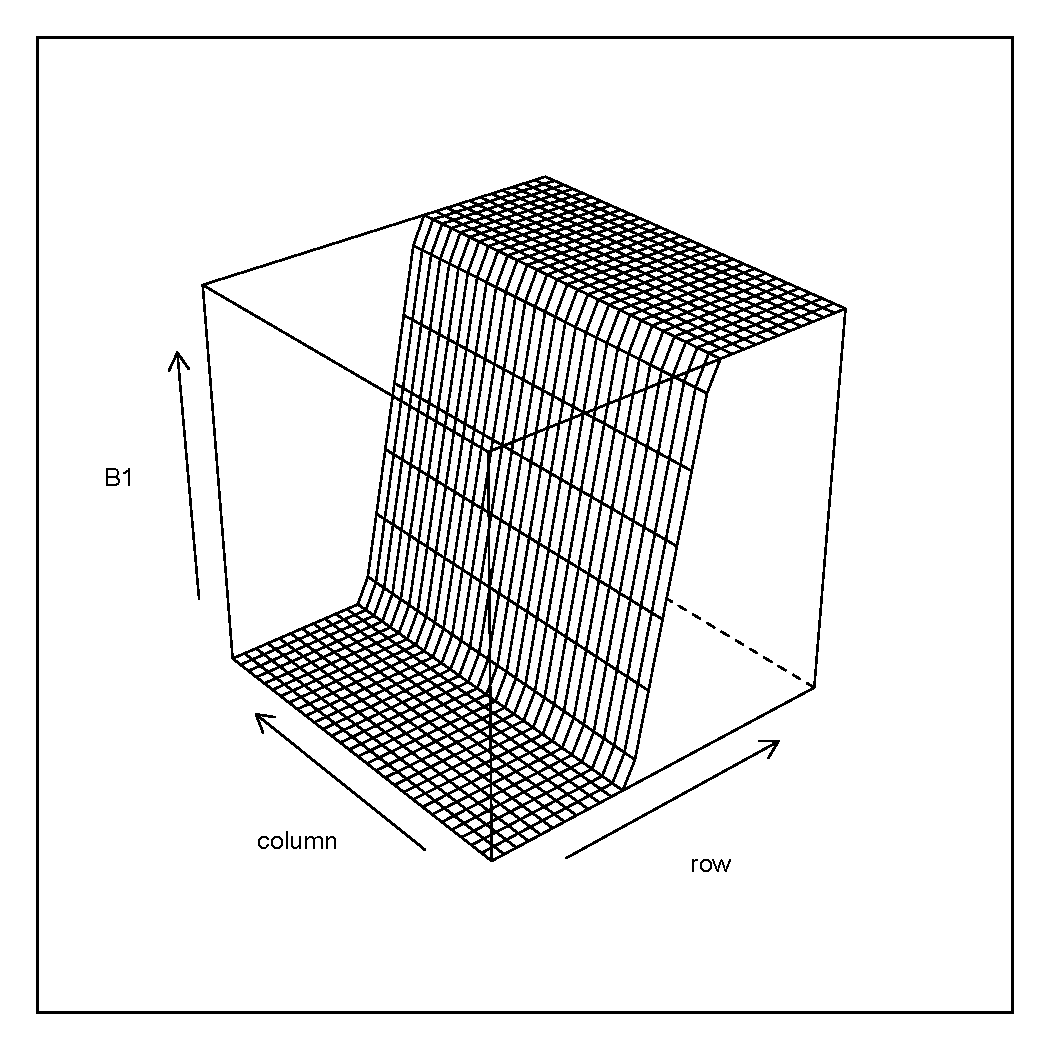
\includegraphics[width=0.33\textwidth]{0_Users_wesley_git_gwr_figures_simulation_step.pdf}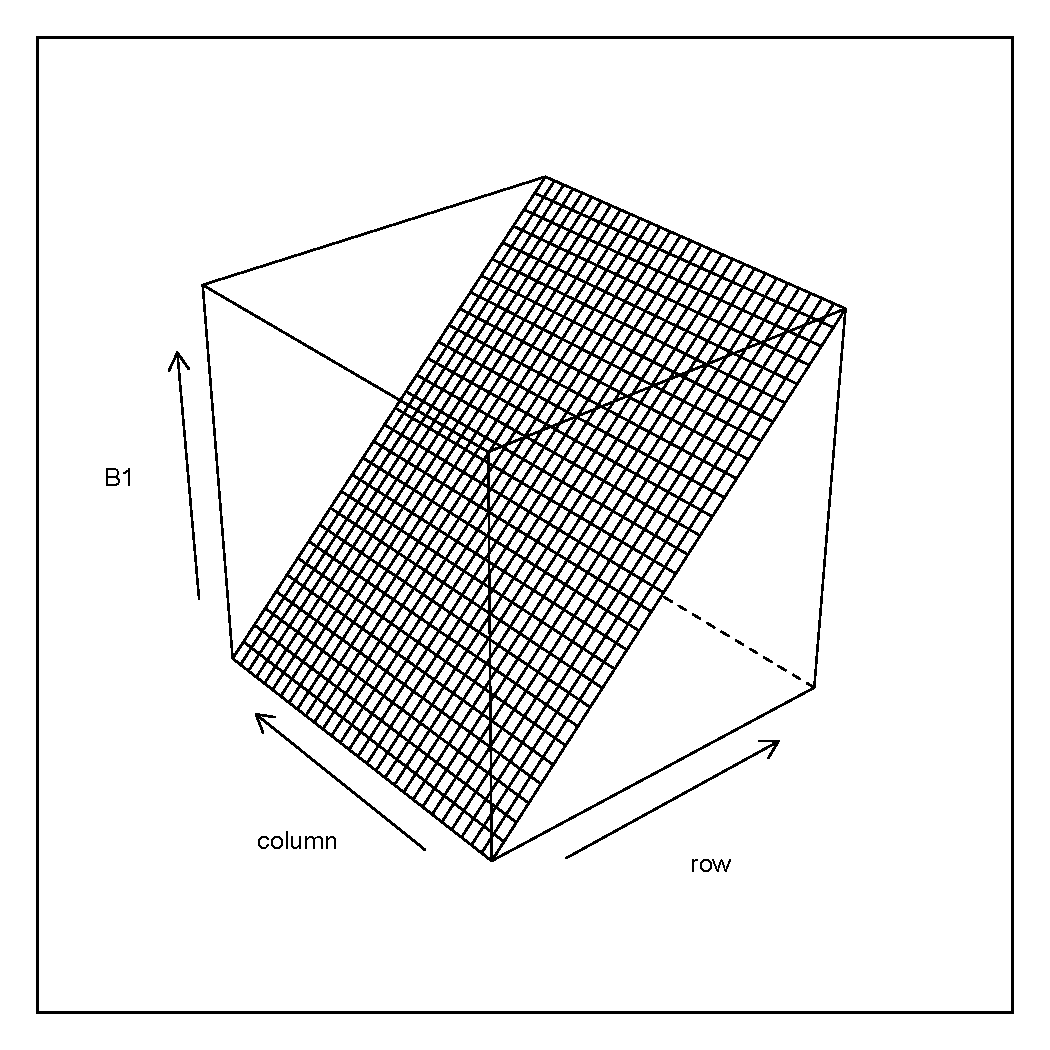
\includegraphics[width=0.33\textwidth]{1_Users_wesley_git_gwr_figures_simulation_gradient.pdf}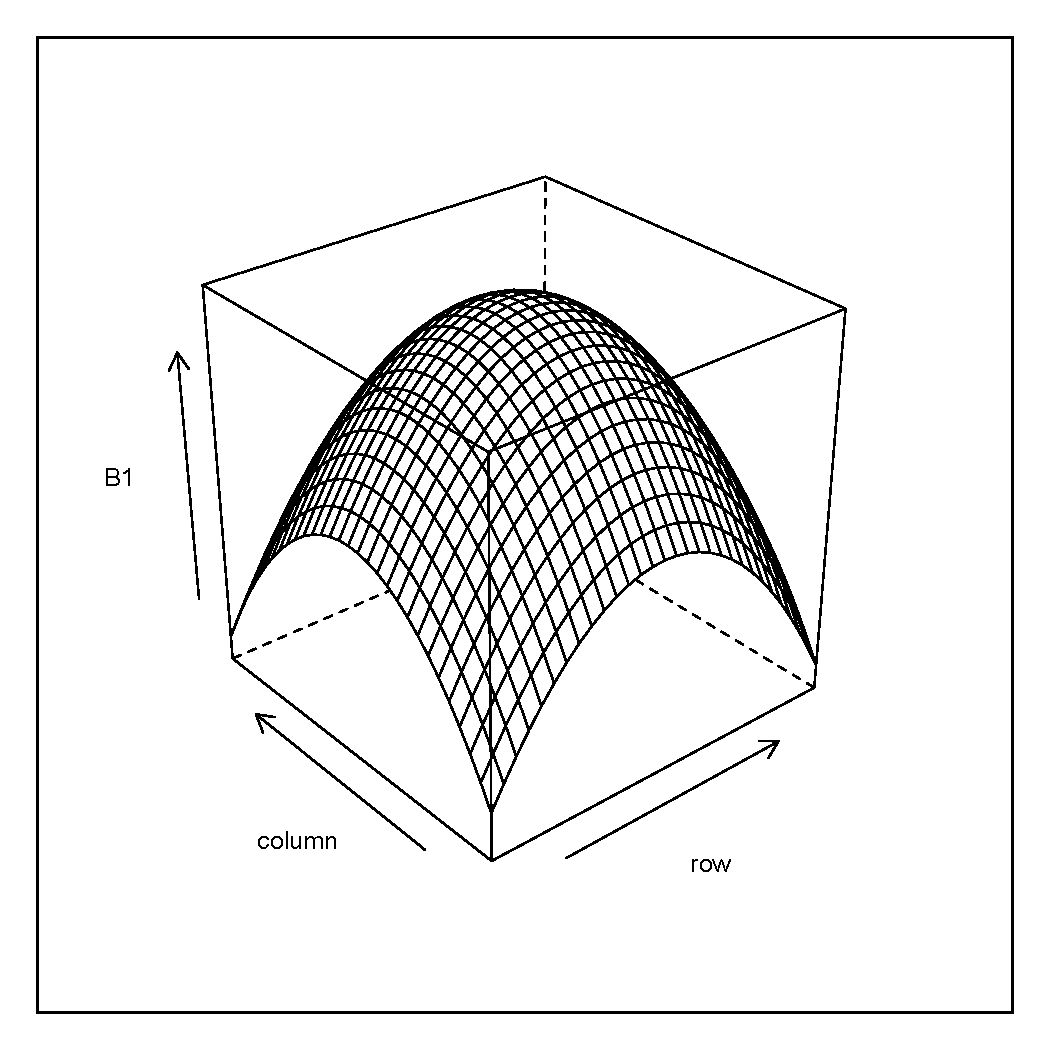
\includegraphics[width=0.33\textwidth]{2_Users_wesley_git_gwr_figures_simulation_parabola.pdf}

\protect\caption{These are, respectively, the step, gradient, and parabola functions
that were used for the coefficient function $\beta_{1}(\bm{s})$ in
the VCR model $y(\bm{s}_{i})=x_{1}(\bm{s}_{i})\beta_{1}(\bm{s}_{i})+\varepsilon(\bm{s}_{i})$
when generating the data for the simulation study.\label{fig:simulation-coefficient-functions}}
\end{figure}


In total, three parameters were varied to produce 18 settings, each
of which was simulated 100 times. There were the three functional
forms for the coefficient surface $\beta_{1}(\bm{s})$; data was simulated
both with low ($\rho=0$), medium ($\rho=0.5$), and high ($\rho=0.9$)
correlation between the covariates; and simulations were made with
low ($\sigma_{\varepsilon}=0.5$) and high ($\sigma_{\varepsilon}=1$)
variance for the random error term.



The results are presented in terms of the mean integrated squared
error (MISE) of the coefficient surface estimates $\hat{\beta}_{1}(\bm{s}),\dots,\hat{\beta}_{5}(\bm{s})$,
the MISE of the fitted response $\hat{y}(\bm{s})$, and the frequency
with which the coefficient surface estimates $\hat{\beta}_{2}(\bm{s}),\dots,\hat{\beta}_{5}(\bm{s})$
estimated by LAGR were zero. The performance of LAGR was compared
to that of a VCR model without variable selection, and to a VCR model
with oracle selection. Oracle selection means that exactly the correct
set of covariates was used to fit each local model.

\begin{table}
	\centering
	\begin{tabular}{ccc|ccc|cc}
		\multicolumn{3}{c}{\begin{tabular}[c]{@{}c@{}}Simulation\\settings\end{tabular}} & \multicolumn{3}{c}{\begin{tabular}[c]{@{}c@{}}MISE\\$\hat{\beta}_1$\end{tabular}} & \multicolumn{2}{c}{\begin{tabular}[c]{@{}c@{}}MISE\\$\hat{\beta}_2, \dots, \hat{\beta}_5$\end{tabular}} \\
		$\beta_{1}(\bm{s})$ & $\rho$ & $\sigma_{\varepsilon}$ & LAGR & VCR & Oracle & LAGR & VCR \\
		\hline 

% latex table generated in R 3.1.1 by xtable 1.7-3 package
% Sun Jul 20 22:08:13 2014
  \multirow{6}{*}{step} & \multirow{2}{*}{0} & 0.5 & \emph{0.02} & 0.02 & \textbf{0.01} & \textbf{0.00} & 0.01 \\ 
    &  & 1.0 & \emph{0.03} & 0.03 & \textbf{0.02} & \textbf{0.00} & 0.02 \\ 
    & \multirow{2}{*}{0.5} & 0.5 & \emph{0.02} & 0.02 & \textbf{0.01} & \textbf{0.00} & 0.01 \\ 
    &  & 1.0 & \emph{0.03} & 0.05 & \textbf{0.02} & \textbf{0.00} & 0.03 \\ 
    & \multirow{2}{*}{0.9} & 0.5 & \emph{0.03} & 0.05 & \textbf{0.01} & \textbf{0.00} & 0.04 \\ 
    &  & 1.0 & \emph{0.12} & 0.17 & \textbf{0.02} & \textbf{0.02} & 0.15 \\ 
   \hline \multirow{6}{*}{gradient} & \multirow{2}{*}{0} & 0.5 & 0.01 & \emph{0.01} & \textbf{0.00} & \textbf{0.00} & 0.00 \\ 
    &  & 1.0 & 0.03 & \emph{0.02} & \textbf{0.01} & \textbf{0.00} & 0.02 \\ 
    & \multirow{2}{*}{0.5} & 0.5 & 0.01 & \emph{0.01} & \textbf{0.00} & \textbf{0.00} & 0.01 \\ 
    &  & 1.0 & 0.04 & \emph{0.03} & \textbf{0.01} & \textbf{0.00} & 0.03 \\ 
    & \multirow{2}{*}{0.9} & 0.5 & \emph{0.03} & 0.04 & \textbf{0.00} & \textbf{0.00} & 0.04 \\ 
    &  & 1.0 & \emph{0.14} & 0.14 & \textbf{0.01} & \textbf{0.02} & 0.15 \\ 
   \hline \multirow{6}{*}{parabola} & \multirow{2}{*}{0} & 0.5 & 0.01 & \emph{0.01} & \textbf{0.01} & \textbf{0.00} & 0.00 \\ 
    &  & 1.0 & 0.03 & \emph{0.02} & \textbf{0.02} & \textbf{0.00} & 0.02 \\ 
    & \multirow{2}{*}{0.5} & 0.5 & 0.01 & \emph{0.01} & \textbf{0.01} & \textbf{0.00} & 0.01 \\ 
    &  & 1.0 & 0.03 & \emph{0.03} & \textbf{0.02} & \textbf{0.00} & 0.03 \\ 
    & \multirow{2}{*}{0.9} & 0.5 & \emph{0.02} & 0.04 & \textbf{0.01} & \textbf{0.00} & 0.04 \\ 
    &  & 1.0 & 0.17 & \emph{0.14} & \textbf{0.02} & \textbf{0.03} & 0.15 \\ 
  

	\end{tabular}
	\caption{Listing of the simulation settings used to assess the performance of LAGR models versus oracle selection and no selection.}
	\label{tab:mise}
\end{table}


\subsection{Simulation Results}

The MISE of the estimates of $\beta_{1}(\bm{s})$ are in Table \ref{tab:misex}.
Recall that $\beta_{2}(\bm{s}),\dots,\beta_{5}(\bm{s})$ are exactly
zero across the entire domain. Oracle selection will estimate these
coefficients perfectly, so we focus on the comparison between estimation
by LAGR and by the VCR model with no selection. These results show
that for every simulation setting, LAGR estimation is more accurate
than the standard VCR model.



From Table \ref{tab:misey} we see that LAGR has good ability to identify
zero-coefficient covariates. The frequency with which $\beta_{2}(\bm{s}),\dots,\beta_{5}(\bm{s})$
were dropped from the LAGR models ranged from 0.78
to 0.97. The MISE of the fitted $\hat{y}(\bm{s})$
is listed in Table \ref{tab:misey}, where the highlighting is based
on which methods estimate an error variance that is closest to the
known truth for the simulation. The results are all very similar to
each other, indicating that no method was consistently better than
the others in this simulation at fitting the model output.

\begin{table}
	\centering
	\begin{tabular}{ccc|c|ccc}
		\multicolumn{3}{c}{\begin{tabular}[c]{@{}c@{}}Simulation\\settings\end{tabular}} &  \multicolumn{1}{c}{\begin{tabular}[c]{@{}c@{}}Zero\\frequency\end{tabular}} &  \multicolumn{3}{c}{\begin{tabular}[c]{@{}c@{}}MISE\\$\hat{y}$\end{tabular}} \\
		$\beta_{1}(\bm{s})$ & $\rho$ & $\sigma_{\varepsilon}$ & $\hat{\beta}_2,\dots,\hat{\beta}_5$ & LAGR & VCR & Oracle \\
		\hline 

% latex table generated in R 3.1.1 by xtable 1.7-3 package
% Sun Jul 20 22:08:15 2014
  \multirow{6}{*}{step} & \multirow{2}{*}{0} & 0.5 & 0.97 & \emph{0.25} & 0.26 & \textbf{0.25} \\ 
    &  & 1.0 & 0.96 & \emph{1.00} & \textbf{1.00} & 0.99 \\ 
    & \multirow{2}{*}{0.5} & 0.5 & 0.96 & \emph{0.26} & 0.26 & \textbf{0.25} \\ 
    &  & 1.0 & 0.92 & \emph{0.99} & \textbf{1.00} & 0.98 \\ 
    & \multirow{2}{*}{0.9} & 0.5 & 0.86 & \emph{0.27} & 0.30 & \textbf{0.25} \\ 
    &  & 1.0 & 0.85 & \emph{1.08} & 1.14 & \textbf{0.98} \\ 
   \hline \multirow{6}{*}{gradient} & \multirow{2}{*}{0} & 0.5 & 0.96 & \emph{0.25} & \textbf{0.25} & 0.25 \\ 
    &  & 1.0 & 0.95 & \textbf{0.99} & \emph{0.99} & 0.97 \\ 
    & \multirow{2}{*}{0.5} & 0.5 & 0.94 & \emph{0.25} & \textbf{0.25} & 0.24 \\ 
    &  & 1.0 & 0.92 & \emph{1.00} & \textbf{1.00} & 0.97 \\ 
    & \multirow{2}{*}{0.9} & 0.5 & 0.80 & \emph{0.27} & 0.28 & \textbf{0.24} \\ 
    &  & 1.0 & 0.85 & \emph{1.09} & 1.12 & \textbf{0.97} \\ 
   \hline \multirow{6}{*}{parabola} & \multirow{2}{*}{0} & 0.5 & 0.97 & \emph{0.25} & \textbf{0.25} & 0.25 \\ 
    &  & 1.0 & 0.94 & \textbf{1.00} & \emph{1.00} & 0.98 \\ 
    & \multirow{2}{*}{0.5} & 0.5 & 0.95 & \textbf{0.25} & 0.25 & \emph{0.25} \\ 
    &  & 1.0 & 0.88 & \textbf{1.00} & \emph{1.00} & 0.97 \\ 
    & \multirow{2}{*}{0.9} & 0.5 & 0.79 & \emph{0.26} & 0.28 & \textbf{0.24} \\ 
    &  & 1.0 & 0.78 & 1.13 & \emph{1.12} & \textbf{0.98} \\ 
  
	\end{tabular}
	\caption{The MISE for the fitted output in each simulation setting, under variable selection via LAGR, no variable selection, and oracular variable selection. Highlighting indicates the \textbf{closest} and \emph{next-closest} to the actual error variance $\sigma_\varepsilon^2$ for that setting.}
	\label{tab:misey}
\end{table}

The proposed LAGR method was accurate in selection and estimation,
with estimation accuracy for $\beta_{1}(\bm{s})$ about equal to that
of the VCR model with no selection, and with consistently better accuracy
for estimating $\beta_{2}(\bm{s}),\dots,\beta_{5}(\bm{s})$.

There was minimal difference in the performance of the proposed LAGR
method between low ($\sigma_{\varepsilon}=0.5$) and high ($\sigma_{\varepsilon}=1$)
error variance, and between no ($\rho=0$) and moderate ($\rho=0.5$)
correlation among the covariates. But the selection and estimation
accuracy did decline when there was high ($\rho=0.9$) correlation
among the covariates.


\section{Data Example\label{sec:example}}




The proposed LAGR estimation method was used to estimate the coefficients
in a VCR model of the effect of some covariates on the price of homes
in Boston based on data from the 1970 U.S. census\citep{Harrison-Rubinfeld-1978,Gilley-Pace-1996,Pace-Gilley-1997}.
The data are the median price of homes sold in 506 census tracts (MEDV),
along with the potential covariates CRIM (the per-capita crime rate
in the tract), RM (the mean number of rooms for houses sold in the
tract), RAD (an index of how accessible the tract is from Boston's
radial roads), TAX (the property tax per \$10,000 of property value),
and LSTAT (the percentage of the tract's residents who are considered
``lower status''). The bandwidth parameter was set to 0.2 for a
nearest neighbors-type bandwidth, meaning that the sum of kernel weights
for each local model was 20\% of the total number of observations.
The kernel used was the Epanechnikov kernel.

A summary of the local coefficients is in Table \ref{tab:boston-coefs-lagr}.
It indicates that RM is the only covariate with a positive mean of
the local coefficients. The coefficient of the CRIM variable was estimated
to be exactly zero at 49\%
of the locations. The percentage for the RAD variable was 37\%.

\begin{figure}

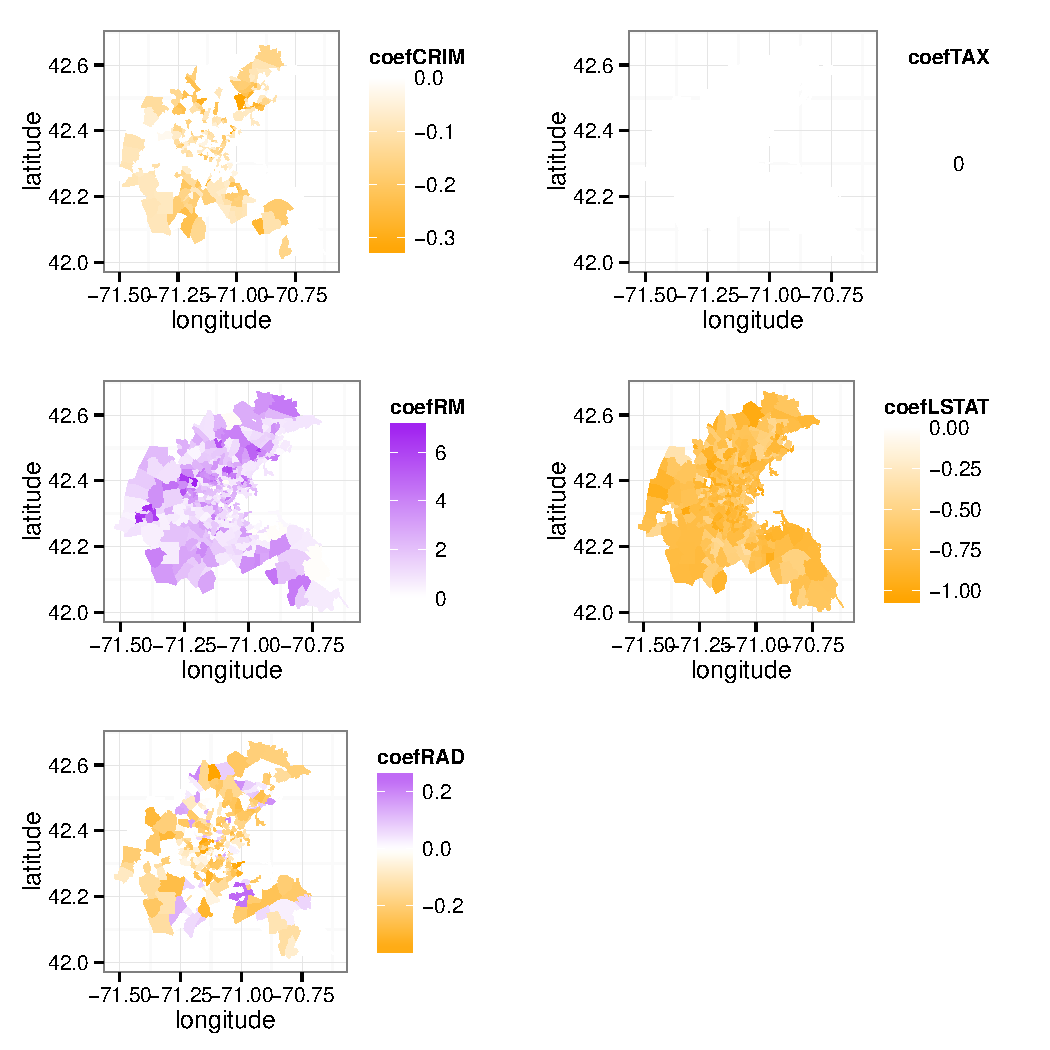
\includegraphics[width=\maxwidth]{figure/boston-plots} 


\caption{The LAGR estimates of coefficients for the Boston house price data.\label{fig:boston-lagr-coefs}}
\end{figure}

Estimates of the regression coefficients are plotted in Figure \ref{fig:boston-lagr-coefs}.
One interesting result is that the TAX variable was nowhere found
to be an important predictor of the median house price. Another is
that the coefficients of CRIM and LSTAT are everywhere negative or
zero (meaning that a greater crime rate or proportion of lower-status
individuals is associated with a lower median house price where the
effect is discernable) and that of RM is positive (meaning that a
greater average number of rooms per house is associated with a greater
median house price). The coefficient of RAD is positive in some areas
and negative in others. This indicates that there are parts of Boston
where access to radial roads is associated with a greater median house
price and parts where it is associated with a lesser median house
price.

% latex table generated in R 3.1.1 by xtable 1.7-3 package
% Sun Jul 20 22:08:23 2014
\begin{table}
\centering
\begin{tabular}{rrrr}
  & Mean & SD & Prop. zero \\ 
  \hline
CRIM & -0.07 & 0.08 & 0.49 \\ 
  RM & 1.92 & 1.43 & 0.02 \\ 
  RAD & -0.08 & 0.13 & 0.37 \\ 
  TAX & 0.00 & 0.00 & 1.00 \\ 
  LSTAT & -0.72 & 0.16 & 0.01 \\ 
  \end{tabular}
\caption{The mean, standard deviation, and proportion of zeros among the local coefficients in a model for the median house price in census tracts in Boston, with coefficients selected and fitted by LAGR.} 
\label{tab:boston-coefs-lagr}
\end{table}


In their example using the same data, \citet{Sun-Yan-Zhang-Lu-2014}
estimated that the coefficients of RAD annd LSTAT should be constant,
at $0.36$ and $-0.45$, respectively. That conclusion differs from
our result, which says that the mean local coefficient of RAD is actually
negative (\ensuremath{-0.08}), while
our mean fitted local coefficient for LSTAT was more negative than
the estimate of \citet{Sun-Yan-Zhang-Lu-2014}.


\section{Extension to GLMs\label{sec:lagr-gllm}}


\subsection{Model}

Generalized linear models (GLMs) extend the linear regression model
to a response variable following any distribution in a single-parameter
exponential family. As was the case for the local linear regression
model, local generalized GLM coefficients are smooth functions of
location. If the response variable $y$ is from an exponential-family
distribution then its density is 

\[
f\left(y\left(\bm{s}\right)|\bm{x}\left(\bm{s}\right),\theta\left(\bm{s}\right)\right)=c\left(y\left(\bm{s}\right)\right)\times\exp\left[\theta\left(\bm{s}\right)y\left(\bm{s}\right)-b\left(\theta\left(\bm{s}\right)\right)\right]
\]


where $\phi$ and $\theta$ are parameters and

\begin{align*}
E\left\{ y(\bm{s})|\bm{x}(\bm{s})\right\} = & \mu(\bm{s})=b'\left(\theta\left(\bm{s}\right)\right)\\
\theta\left(\bm{s}\right)= & (g\circ b')^{-1}\left(\eta\left(\bm{s}\right)\right)\\
\eta\left(\bm{s}\right)= & \bm{x}^{T}\left(\bm{s}\right)\bm{\beta}\left(\bm{s}\right)=g\left(\mu\left(\bm{s}\right)\right)\\
\text{\text{Var}}\left\{ y\left(\bm{s}\right)|\bm{x}\left(\bm{s}\right)\right\} = & b''\left(\theta\left(\bm{s}\right)\right)
\end{align*}


The function $g(\cdot)$ is called the link function. If its inverse
$g^{-1}(\cdot)=b'(\cdot)$, then the composition $\left(g\circ b'\right)\left(\cdot\right)$
is the identity function. This particular $g$ is called the canonical
link. 


\subsection{Local quasi-likelihood}

Assuming the canonical link, all that is required is to specify the
mean-variance relationship via the variance function, $V\left(\mu\left(\bm{s}\right)\right)$.
Then the local coefficients can be estimated by maximizing the local
quasi-likelihood 

\begin{align}
\mathcal{\ell}^{*}\left(\bm{\zeta}(\bm{s})\right) & =\sum_{i=1}^{n}K_{h}\left(\|\bm{s}-\bm{s}_{i}\|\right)Q\left(g^{-1}\left(\bm{z}_{i}^{T}\bm{\zeta}(\bm{s})\right),Y_{i}\right),
\end{align}


where $\bm{Z}\left(\bm{s}\right)$ and $\bm{\zeta}\left(\bm{s}\right)$
are defined in (\ref{eq:augmented-covariates}) and (\ref{eq:augmented-coefficients}).
The local quasi-likelihood generalizes the local log-likelihood that
was used to estimate coefficients in the local linear model case.
The quasi-likelihood is convex, and is defined in terms of its derivative,
the quasi-score function

\[
\frac{\partial}{\partial\mu}Q\left(\mu,y\right)=\frac{y-\mu}{V\left(\mu\right)}.
\]



\subsection{Estimation}

Under these conditions, the local quasi-likelihood is maximized where

\begin{align}
\frac{\partial}{\partial\bm{\zeta}}\mathcal{\ell}^{*}\left(\hat{\bm{\zeta}}\left(\bm{s}\right)\right) & =\sum_{i=1}^{n}K_{h}\left(\|\bm{s}-\bm{s}_{i}\|\right)\frac{y_{i}-\hat{\mu}\left(\bm{s}_{i};\bm{s}\right)}{V\left(\hat{\mu}\left(\bm{s}_{i};\bm{s}\right)\right)}\bm{z}_{i}=\bm{0}_{3p}
\end{align}


and $\hat{\mu}\left(\bm{s}_{i};\bm{s}\right)=g^{-1}\left(\bm{z}_{i}^{T}\hat{\bm{\zeta}}\left(\bm{s}\right)\right)$
is the mean at location $\bm{s}_{i}$ estimated using the coefficients
$\hat{\bm{\zeta}}\left(\bm{s}\right)$ fitted at location $\bm{s}$.
The asymptotic distribution of the local coefficients in a varying-coefficient
GLM with a one-dimensional effect-modifying parameter are given in
\citet{Cai-Fan-Li-2000}. For coefficients that vary in two dimensions,
the distribution of the estimated local coefficients is (see Lemmas
\ref{lemma:omega} and \ref{lemma:delta})

\[
\sqrt{{nh^{2}f(\bm{{s}})}}\left[\tilde{\bm{\beta}}(\bm{s})-\bm{\beta}(\bm{s})-(1/2)\kappa_{0}^{-1}\kappa_{2}h^{2}\left\{ \nabla_{uu}^{2}\bm{\beta}(\bm{s})+\nabla_{vv}^{2}\bm{\beta}(\bm{s})\right\} \right]\xrightarrow{{D}}N\left(\bm{0},\kappa_{0}^{-2}\nu_{0}\Gamma^{-1}(\bm{s})\right).
\]



\subsection{LAGR penalty}

As in the case of linear models, the LAGR for GLMs is a grouped $\ell_{1}$
regularization method. Now, though, we use a penalized local quasi-likelihood:

\begin{align}
\mathcal{J}\left(\bm{\zeta}(\bm{s})\right) & =\mathcal{\ell}^{*}\left(\bm{\zeta}(\bm{s})\right)+\mathcal{P}\left(\bm{\zeta}(\bm{s})\right)\label{eq:adaptive-lasso-GLLM}\\
 & =\sum_{i=1}^{n}K_{h}\left(\|\bm{s}-\bm{s}_{i}\|\right)Q\left(g^{-1}\left(\bm{z}_{i}^{T}\bm{\zeta}(\bm{s})\right),Y_{i}\right)+\sum_{j=1}^{p}\phi_{j}\left(\bm{s}\right)\|\bm{\zeta}_{\left(j\right)}\left(\bm{s}\right)\|
\end{align}


and, as in the case of gaussian data, $\phi_{j}\left(\bm{s}\right)=\lambda_{n}\|\tilde{\bm{\zeta}}_{\left(j\right)}\left(\bm{s}\right)\|^{-\gamma}$,
where $\lambda_{n}>0$ is a the local tuning parameter applied to
all coefficients at location $\bm{s}$ and $\tilde{\bm{\zeta}}_{\left(j\right)}\left(\bm{s}\right)$
is the vector of unpenalized local coefficients.


\subsection{Oracle properties of LAGR in the GLM setting}

The following are additional to the definitions and assumptions of
Section \ref{sub:oracle-properties}:

Define
\begin{itemize}
\item[(D.5)] Let $\rho\left(\bm{s},\bm{z}\right)=\left[g_{1}\left(\mu\left(\bm{s},\bm{z}\right)\right)\right]^{2}Var\left\{ Y\left(\bm{s}\right)|\bm{X}\left(\bm{s}\right),\bm{s}\right\} $,
where $g_{1}\left(\cdot\right)=g'_{0}\left(\cdot\right)/g'\left(\cdot\right)$,
and $g_{0}\left(\cdot\right)$ is the canonical link function. So
when the canonical link is used, $\rho\left(\bm{s},\bm{z}\right)=V\left(\mu\left(\bm{s},\bm{z}\right)\right)$.
\item[(D.6)] Let $\Gamma\left(\bm{s}\right)=E\left\{ \rho\left(\bm{s},\bm{X}\left(\bm{s}\right)\right)\bm{X}\left(\bm{s}\right)\bm{X}\left(\bm{s}\right)^{T}|\bm{s},\bm{Z}\left(\bm{s}\right)=\bm{z}\right\} $.
\end{itemize}
Assume the following conditions.
\begin{itemize}
\item[(A.9)] The functions $g'''\left(\bm{s}\right)$, $\Gamma\left(\bm{s}\right)$,
$V\left(\mu\left(\bm{s},\bm{z}\right)\right)$, and $V'\left(\mu\left(\bm{s},\bm{z}\right)\right)$
are continuous at the point $\bm{s}$.
\item[(A.10)] The function $\left(\partial^{2}/\partial\mu^{2}\right)Q\left(g^{-1}\left(\mu\right),y\right)<0$
for $\mu\in\mathbb{R}$ and $y$ in the range of the response variable.
\end{itemize}
Then,
\begin{thm}[Asymptotic normality]
\label{theorem:normality-glm} 



If $h^{-1}n^{-1/2}a_{n}\xrightarrow{p}0$ and $hn^{-1/2}b_{n}\xrightarrow{p}\infty$
then 
\[
\sqrt{nh^{2}f\left(\bm{s}\right)}\left[\hat{\bm{\beta}}_{a}(\bm{s})-\bm{\beta}_{a}(\bm{s})-\frac{\kappa_{2}h^{2}}{2\kappa_{0}}\left\{ \nabla_{uu}^{2}\bm{\beta}_{a}(\bm{s})+\nabla_{vv}^{2}\bm{\beta}_{a}(\bm{s})\right\} \right]\xrightarrow{d}N\left(0,\kappa_{0}^{-2}\nu_{0}\Gamma^{-1}(\bm{s})\right)
\]

\end{thm}

\begin{thm}[Selection consistency]
\label{theorem:selection-glm}



If $h^{-1}n^{-1/2}a_{n}\xrightarrow{p}0$ and $hn^{-1/2}b_{n}\xrightarrow{p}\infty$
then $Pr\left\{ \|\hat{\bm{\zeta}}_{j}(\bm{s})\|=\utilde{0}\right\} \to0$
if $j\le p_{0}$ and $Pr\left\{ \|\hat{\bm{\zeta}}_{j}(\bm{s})\|=\utilde{0}\right\} \to1$
if $j>p_{0}$. 
\end{thm}
\appendix

\section*{Appendix: Proof of Theorem \ref{theorem:normality}\label{sec:gaussian-normality-proof} }
\begin{proof}
Let $H_{n}(\bm{u})=\mathcal{J}\left(\bm{\zeta}\left(\bm{s}\right)+h^{-1}n^{-1/2}\bm{u}\right)-\mathcal{J}\left(\bm{\zeta}\left(\bm{s}\right)\right)$
and $\alpha_{n}=h^{-1}n^{-1/2}$. Then, we have 
\begin{align*}
H_{n}\left(\bm{u}\right)= & (1/2)\left[\bm{Y}-\bm{Z}(\bm{s})\left\{ \bm{\zeta}\left(\bm{s}\right)+\alpha_{n}\bm{u}\right\} \right]^{T}\bm{W}(\bm{s})\left[\bm{Y}-\bm{Z}(\bm{s})\left\{ \bm{\zeta}\left(\bm{s}\right)+\alpha_{n}\bm{u}\right\} \right]\\
 & +\sum_{j=1}^{p}\phi_{j}(\bm{s})\|\bm{\zeta}_{j}(\bm{s})+\alpha_{n}\bm{u}_{j}\|\\
 & -(1/2)\left\{ \bm{Y}-\bm{Z}(\bm{s})\bm{\zeta}(\bm{s})\right\} ^{T}\bm{W}(\bm{s})\left\{ \bm{Y}-\bm{Z}(\bm{s})\bm{\zeta}(\bm{s})\right\} -\sum_{j=1}^{p}\phi_{j}(\bm{s})\|\bm{\zeta}_{j}(\bm{s})\|\\
= & \left(1/2\right)\alpha_{n}^{2}\bm{u}^{T}\left\{ \bm{Z}^{T}(\bm{s})\bm{W}(\bm{s})\bm{Z}(\bm{s})\right\} \bm{u}\\
 & -\alpha_{n}\bm{u}^{T}\left[\bm{Z}^{T}(\bm{s})\bm{W}(\bm{s})\left\{ \bm{Y}-\bm{Z}(\bm{s})\bm{\zeta}(\bm{s})\right\} \right]\\
 & +\sum_{j=1}^{p}n^{-1/2}\phi_{j}(\bm{s})n^{1/2}\left\{ \|\bm{\zeta}_{\left(j\right)}(\bm{s})+\alpha_{n}\bm{u}_{\left(j\right)}\|-\|\bm{\zeta}_{\left(j\right)}(\bm{s})\|\right\} 
\end{align*}


The limiting behavior of the last term differs between the cases $j\le p_{0}$
and $j>p_{0}$.

\emph{Case $j\le p_{0}$}: If $j\le p_{0}$, then $n^{-1/2}\phi_{j}(\bm{s})\to n^{-1/2}\lambda_{n}\|\bm{\zeta}_{\left(j\right)}(\bm{s})\|^{-\gamma}$
and $|\sqrt{n}\left\{ \|\bm{\zeta}_{\left(j\right)}(\bm{s})+\alpha_{n}\bm{u}_{\left(j\right)}\|-\|\bm{\zeta}_{\left(j\right)}(\bm{s})\|\right\} |\le h^{-1}\|\bm{u}_{\left(j\right)}\|$
. Thus, 
\[
\phi_{j}(\bm{s})\left(\|\bm{\zeta}_{\left(j\right)}(\bm{s})+\alpha_{n}\bm{u}_{\left(j\right)}\|-\|\bm{\zeta}_{\left(j\right)}(\bm{s})\|\right)\le\alpha_{n}\phi_{j}(\bm{s})\|\bm{u}_{\left(j\right)}\|\le\alpha_{n}a_{n}\|\bm{u}_{\left(j\right)}\|\to0
\]


\emph{Case $j>p_{0}$}: If $j>p_{0}$, then $\phi_{j}(\bm{s})\left(\|\bm{\zeta}_{\left(j\right)}(\bm{s})+\alpha_{n}\bm{u}_{\left(j\right)}\|-\|\bm{\zeta}_{\left(j\right)}(\bm{s})\|\right)=\phi_{j}(\bm{s})\alpha_{n}\|\bm{u}_{\left(j\right)}\|$.
Since $h=O(n^{-1/6})$, if $hn^{-1/2}b_{n}\xrightarrow{p}\infty$,
then $\alpha_{n}b_{n}\xrightarrow{p}\infty$. Thus, if $\|\bm{u}_{\left(j\right)}\|\ne0$,
then 
\[
\alpha_{n}\phi_{j}(\bm{s})\|\bm{u}_{\left(j\right)}\|\ge\alpha_{n}b_{n}\|\bm{u}_{\left(j\right)}\|\to\infty.
\]
On the other hand, if $\|\bm{u}_{\left(j\right)}\|=0$, then $\alpha_{n}\phi_{j}(\bm{s})\|\bm{u}_{\left(j\right)}\|=0$.

Thus, the limit of $H_{n}\left(\bm{u}\right)$ is the same as the
limit of $H_{n}^{*}\left(\bm{u}\right)$ where $H_{n}^{*}\left(\bm{u}\right)=\infty$
if $\exists j>p_{0}\ s.t.\ \|\bm{u}_{\left(j\right)}\|\ne0$, and 

\[
H_{n}^{*}\left(\bm{u}\right)=(1/2)\alpha_{n}^{2}\bm{u}^{T}\left\{ \bm{Z}^{T}(\bm{s})\bm{W}(\bm{s})\bm{Z}(\bm{s})\right\} \bm{u}-\alpha_{n}\bm{u}^{T}\left[\bm{Z}^{T}(\bm{s})\bm{W}(\bm{s})\left\{ \bm{Y}-\bm{Z}(\bm{s})\bm{\zeta}(\bm{s})\right\} \right]
\]


otherwise. It follows that $H_{n}^{*}\left(\bm{u}\right)$ is convex
and its unique minimizer is 
\[
\hat{\bm{u}}_{n}=\left\{ n^{-1}\bm{Z}^{T}\left(\bm{s}\right)\bm{W}\left(\bm{s}\right)\bm{Z}\left(\bm{s}\right)\right\} ^{-1}\left[hn^{1/2}\bm{Z}\left(\bm{s}\right)^{T}\bm{W}\left(\bm{s}\right)\left\{ \bm{Y}-\bm{Z}\left(\bm{s}\right)\bm{\zeta}\left(\bm{s}\right)\right\} \right].
\]
By epiconvergence, the minimizer of the limiting function is the limit
of the minimizers $\hat{\bm{u}}_{n}$ \citep{Geyer-1994,Knight-Fu-2000}.
Since, by Lemma 2 of \citet{Sun-Yan-Zhang-Lu-2014},

\[
\hat{\bm{u}}_{n}-\alpha_{n}^{-1}f\left(\bm{s}\right)^{-1/2}2^{-1}\kappa_{0}^{-1}\kappa_{2}h^{2}\left\{ \nabla_{uu}^{2}\bm{\zeta}(\bm{s})+\nabla_{vv}^{2}\bm{\zeta}(\bm{s})\right\} \xrightarrow{d}N\left(0,\alpha_{n}^{-2}f\left(\bm{s}\right)^{-1}\kappa_{0}^{-2}\nu_{0}\sigma^{2}\Psi\left(\bm{s}\right)^{-1}\right)
\]
the result of Theorem \ref{theorem:normality} follows.
\end{proof}

\section*{Appendix: Proof of Theorem \ref{theorem:selection}\label{sec:gaussian-selection-proof}}
\begin{proof}
We showed in Theorem \ref{theorem:normality} that $\hat{\bm{\zeta}}_{\left(j\right)}\left(\bm{s}\right)\xrightarrow{p}\bm{\zeta}_{\left(j\right)}\left(\bm{s}\right)+\frac{\kappa_{2}h^{2}}{2\kappa_{0}}\{\nabla_{uu}^{2}\bm{\zeta}_{\left(j\right)}\left(\bm{s}\right)+\nabla_{vv}^{2}\bm{\zeta}_{\left(j\right)}\left(\bm{s}\right)\}$,
so to complete the proof of selection consistency, it only remains
to show that $Pr\left\{ \hat{\bm{\zeta}}_{\left(j\right)}\left(\bm{s}\right)=\utilde{0}\right\} \to1$
if $j>p_{0}$.

The proof is by contradiction. Without loss of generality we consider
only the case $j=p$.

Assume $\|\hat{\bm{\zeta}}_{\left(p\right)}(\bm{s})\|\ne0$. Then
$\mathcal{J}\left(\bm{\zeta}\left(\bm{s}\right)\right)$ is differentiable
w.r.t. $\bm{\zeta}_{\left(p\right)}\left(\bm{s}\right)$ and is minimized
where 
\begin{align*}
\utilde{0}= & \bm{Z}_{\left(p\right)}^{T}\left(\bm{s}\right)\bm{W}\left(\bm{s}\right)\left\{ \bm{Y}-\bm{Z}_{\left(-p\right)}\left(\bm{s}\right)\hat{\bm{\zeta}}_{\left(-p\right)}\left(\bm{s}\right)-\bm{Z}_{\left(p\right)}\left(\bm{s}\right)\hat{\bm{\zeta}}_{\left(p\right)}\left(\bm{s}\right)\right\} -\phi_{\left(p\right)}(\bm{s})\frac{\hat{\bm{\zeta}}_{\left(p\right)}\left(\bm{s}\right)}{\|\hat{\bm{\zeta}}_{\left(p\right)}\left(\bm{s}\right)\|}\\
= & \bm{Z}_{\left(p\right)}\left(\bm{s}\right)^{T}\bm{W}\left(\bm{s}\right)\left[\bm{Y}-\bm{Z}\left(\bm{s}\right)\bm{\zeta}\left(\bm{s}\right)-\frac{h^{2}\kappa_{2}}{2\kappa_{0}}\left\{ \nabla_{uu}^{2}\bm{\zeta}\left(\bm{s}\right)+\nabla_{vv}^{2}\bm{\zeta}\left(\bm{s}\right)\right\} \right]\\
 & +\bm{Z}_{\left(p\right)}\left(\bm{s}\right)^{T}\bm{W}\left(\bm{s}\right)\bm{Z}_{\left(-p\right)}\left(\bm{s}\right)\left[\bm{\zeta}_{\left(-p\right)}\left(\bm{s}\right)+\frac{h^{2}\kappa_{2}}{2\kappa_{0}}\left\{ \nabla_{uu}^{2}\bm{\zeta}_{\left(-p\right)}\left(\bm{s}\right)+\nabla_{vv}^{2}\bm{\zeta}_{\left(-p\right)}\left(\bm{s}\right)\right\} -\hat{\bm{\zeta}}_{-\left(p\right)}\left(\bm{s}\right)\right]\\
 & +\bm{Z}_{\left(p\right)}\left(\bm{s}\right)^{T}\bm{W}\left(\bm{s}\right)\bm{Z}_{\left(p\right)}\left(\bm{s}\right)\left[\bm{\zeta}_{\left(p\right)}\left(\bm{s}\right)+\frac{h^{2}\kappa_{2}}{2\kappa_{0}}\left\{ \nabla_{uu}^{2}\bm{\zeta}_{\left(p\right)}\left(\bm{s}\right)+\nabla_{vv}^{2}\bm{\zeta}_{\left(p\right)}\left(\bm{s}\right)\right\} -\hat{\bm{\zeta}}_{\left(p\right)}\left(\bm{s}\right)\right]\\
 & -\phi_{p}\left(\bm{s}\right)\frac{\hat{\bm{\zeta}}_{\left(p\right)}\left(\bm{s}\right)}{\|\hat{\bm{\zeta}}_{\left(p\right)}\left(\bm{s}\right)\|}
\end{align*}


Thus, 
\begin{align}
\frac{h}{\sqrt{n}} & \phi_{p}\left(\bm{s}\right)\frac{\hat{\bm{\zeta}}_{\left(p\right)}\left(\bm{s}\right)}{\|\hat{\bm{\zeta}}_{\left(p\right)}\left(\bm{s}\right)\|}=\nonumber \\
 & \bm{Z}_{\left(p\right)}\left(\bm{s}\right)^{T}\bm{W}\left(\bm{s}\right)\frac{h}{\sqrt{n}}\left[\bm{Y}-\bm{Z}\left(\bm{s}\right)\bm{\zeta}\left(\bm{s}\right)-\frac{h^{2}\kappa_{2}}{2\kappa_{0}}\left\{ \nabla_{uu}^{2}\bm{\zeta}\left(\bm{s}\right)+\nabla_{vv}^{2}\bm{\zeta}\left(\bm{s}\right)\right\} \right]\nonumber \\
 & +\left\{ n^{-1}\bm{Z}_{\left(p\right)}\left(\bm{s}\right)^{T}\bm{W}(\bm{s})\bm{Z}_{\left(-p\right)}\left(\bm{s}\right)\right\} \sqrt{nh^{2}}\left[\bm{\zeta}_{\left(-p\right)}\left(\bm{s}\right)+\frac{h^{2}\kappa_{2}}{2\kappa_{0}}\left\{ \nabla_{uu}^{2}\bm{\zeta}_{\left(-p\right)}\left(\bm{s}\right)+\nabla_{vv}^{2}\bm{\zeta}_{\left(-p\right)}\left(\bm{s}\right)\right\} -\hat{\bm{\zeta}}_{\left(-p\right)}\left(\bm{s}\right)\right]\nonumber \\
 & +\left\{ n^{-1}\bm{Z}_{\left(p\right)}\left(\bm{s}\right)^{T}\bm{W}\left(\bm{s}\right)\bm{Z}_{\left(p\right)}\left(\bm{s}\right)\right\} \sqrt{nh^{2}}\left[\bm{\zeta}_{\left(p\right)}\left(\bm{s}\right)+\frac{h^{2}\kappa_{2}}{2\kappa_{0}}\left\{ \nabla_{uu}^{2}\bm{\zeta}_{\left(p\right)}\left(\bm{s}\right)+\nabla_{vv}^{2}\bm{\zeta}_{\left(p\right)}\left(\bm{s}\right)\right\} -\hat{\bm{\zeta}}_{\left(p\right)}\left(\bm{s}\right)\right]\label{eq:selection}
\end{align}


From Lemma 2 of \citet{Sun-Yan-Zhang-Lu-2014}, 
\[
O_{p}\left(n^{-1}\bm{Z}_{\left(p\right)}\!\left(\bm{s}\right)^{T}\bm{W}\!\left(\bm{s}\right)\bm{Z}_{\left(-p\right)}\!\left(\bm{s}\right)\right)=O_{p}\left(n^{-1}\bm{Z}_{\left(p\right)}\!\left(\bm{s}\right)^{T}\bm{W}\!\left(\bm{s}\right)\bm{Z}_{\left(p\right)}\!\left(\bm{s}\right)\right)=O_{p}\left(1\right).
\]


From Theorem 3 of \citet{Sun-Yan-Zhang-Lu-2014}, we have that 
\[
\sqrt{nh^{2}}\left[\hat{\bm{\zeta}}_{\left(-p\right)}\left(\bm{s}\right)-\bm{\zeta}_{\left(-p\right)}\left(\bm{s}\right)-\frac{h^{2}\kappa_{2}}{2\kappa_{0}}\left\{ \nabla_{uu}^{2}\zeta_{\left(-p\right)}\left(\bm{s}\right)+\nabla_{vv}^{2}\zeta_{\left(-p\right)}\left(\bm{s}\right)\right\} \right]=O_{p}\left(1\right)
\]
 and 
\[
\sqrt{nh^{2}}\left[\hat{\bm{\zeta}}_{\left(p\right)}\left(\bm{s}\right)-\bm{\zeta}_{\left(p\right)}\left(\bm{s}\right)-\frac{h^{2}\kappa_{2}}{2\kappa_{0}}\left\{ \nabla_{uu}^{2}\bm{\zeta}_{\left(p\right)}\left(\bm{s}\right)+\nabla_{vv}^{2}\bm{\zeta}_{\left(p\right)}\left(\bm{s}\right)\right\} \right]=O_{p}\left(1\right).
\]


We showed in the proof of Theorem \ref{theorem:normality} that

\[
\sqrt{nh^{2}}\bm{Z}_{\left(p\right)}\left(\bm{s}\right)^{T}\bm{W}\left(\bm{s}\right)\left[\bm{Y}-\bm{Z}\left(\bm{s}\right)\bm{\zeta}\left(\bm{s}\right)-\frac{h^{2}\kappa_{2}}{2\kappa_{0}}\left\{ \nabla_{uu}^{2}\bm{\zeta}\left(\bm{s}\right)+\nabla_{vv}^{2}\bm{\zeta}\left(\bm{s}\right)\right\} \right]=O_{p}\left(1\right).
\]


The right hand side of (\ref{eq:selection}) is $O_{p}(1)$, so for
$\hat{\bm{\zeta}}_{\left(p\right)}\left(\bm{s}\right)$ to be a solution,
we must have that $hn^{-1/2}\phi_{p}\left(\bm{s}\right)\hat{\bm{\zeta}}_{\left(p\right)}\left(\bm{s}\right)/\|\hat{\bm{\zeta}}_{\left(p\right)}\left(\bm{s}\right)\|=O_{p}\left(1\right)$.

But since by assumption $\hat{\bm{\zeta}}_{\left(p\right)}\left(\bm{s}\right)\ne\utilde{0}$,
there must be some $k\in\{1,2,3\}$ such that $|\hat{\zeta}_{\left(p\right)_{k}}\left(\bm{s}\right)|=\max\{|\hat{\zeta}_{\left(p\right)_{m}}\left(\bm{s}\right)|:1\le m\le3\}$.
And for this $k$, we have that $|\hat{\zeta}_{\left(p\right)_{k}}\left(\bm{s}\right)|/\|\hat{\bm{\zeta}}_{\left(p\right)}\left(\bm{s}\right)\|\ge1/\sqrt{3}>0$.

Since $hn^{-1/2}b_{n}\to\infty$, we have that $hn^{-1/2}\phi_{p}\left(\bm{s}\right)\hat{\bm{\zeta}}_{\left(p\right)}\left(\bm{s}\right)/\|\hat{\bm{\zeta}}_{\left(p\right)}\left(\bm{s}\right)\|\ge hb_{n}/\sqrt{3n}\to\infty$
and therefore the left hand side of (\ref{eq:selection}) dominates
the sum to the right side. Thus, for large enough $n$, $\hat{\bm{\zeta}}_{\left(p\right)}\left(\bm{s}\right)\ne\utilde{0}$
cannot maximize $\mathcal{J}\left(\cdot\right)$, and therefore $Pr\left\{ \hat{\bm{\zeta}}_{(b)}\left(\bm{s}\right)=\utilde{0}\right\} \to1$. 
\end{proof}

\section*{Appendix: Lemmas}

The next proofs require the following lemmas. First, we define the
following terms:
\begin{itemize}
\item[(D.A.1)] Let $\bm{x}\in\mathbb{R}^{3p}$
\item[(D.A.2)] Define the $q$-functions to be the derivatives of the quasi-likelihood:
$q_{j}(t,y)=\left(\partial/\partial t\right)^{j}Q\left(g^{-1}\left(t\right),y\right)$.
Then

\begin{itemize}
\item (a) $q_{1}\left(\eta\left(\bm{s},\bm{x}\right),\mu\left(\bm{s},\bm{x}\right)\right)=\utilde{0}$,
and 
\item (b) $q_{2}\left(\eta\left(\bm{s},\bm{x}\right),\mu\left(\bm{s},\bm{x}\right)\right)=-\rho\left(\bm{s},\bm{x}\right)$.
\end{itemize}
\item[(D.A.3)] Let $\tilde{\bm{\zeta}}_{i}''=\left[\left(\bm{s}_{i}-\bm{s}\right)^{T}\left\{ \nabla^{2}\zeta_{1}\left(\bm{s}\right)\right\} \left(\bm{s}_{i}-\bm{s}\right),\dots,\left(\bm{s}_{i}-\bm{s}\right)^{T}\left\{ \nabla^{2}\zeta_{3p}\left(\bm{s}\right)\right\} \left(\bm{s}_{i}-\bm{s}\right)\right]^{T}$
be the $3p$-vector of quadratic forms of location interactions on
the second derivatives of the coefficient functions.\end{itemize}
\begin{lem}
\label{lemma:omega}

\begin{multline*}
E\left[\sum_{i=1}^{n}q_{1}\left(\bm{Z}_{i}^{T}\bm{\zeta}\left(\bm{s}\right),Y_{i}\right)\bm{Z}_{i}K_{h}\left(\|\bm{s}-\bm{s}_{i}\|\right)\right]=\\
\left(\begin{array}{c}
2^{-1}n^{1/2}h^{3}\kappa_{2}f\left(\bm{s}\right)\Gamma\left(\bm{s}\right)\left(\nabla_{uu}^{2}\bm{\beta}\left(\bm{s}\right)+\nabla_{vv}^{2}\bm{\beta}\left(\bm{s}\right)\right)^{T}\\
\bm{0}_{2p}
\end{array}\right)+o_{p}\left(h^{2}\bm{1}_{3p}\right)
\end{multline*}


and 

\begin{align*}
\end{align*}


\begin{align*}
Var\left[\sum_{i=1}^{n}q_{1}\left(\bm{Z}_{i}^{T}\bm{\zeta}\left(\bm{s}\right),Y_{i}\right)\bm{Z}_{i}K_{h}\left(\|\bm{s}-\bm{s}_{i}\|\right)\right]= & f\left(\bm{s}\right)diag\left\{ \nu_{0},\nu_{2},\nu_{2}\right\} \otimes\Gamma\left(\bm{s}\right)+o\left(1\right)\\
= & \Lambda+o\left(1\right)
\end{align*}

\end{lem}

\begin{lem}
\label{lemma:delta}

\begin{align*}
E\left[\sum_{i=1}^{n}q_{2}\left(\bm{Z}_{i}^{T}\bm{\zeta}\left(\bm{s}\right),Y_{i}\right)\bm{Z}_{i}\bm{Z}_{i}^{T}K_{h}\left(\|\bm{s}-\bm{s}_{i}\|\right)\right]= & -f\left(\bm{s}\right)diag\left\{ \kappa_{0},\kappa_{2},\kappa_{2}\right\} \otimes\Gamma\left(\bm{s}\right)+o\left(1\right)\\
= & -\Delta+o\left(1\right)
\end{align*}


\begin{multline*}
\\
\end{multline*}


and

\[
Var\left\{ \left(\sum_{i=1}^{n}q_{2}\left(\bm{Z}_{i}^{T}\bm{\zeta}\left(\bm{s}\right),Y_{i}\right)\bm{Z}_{i}\bm{Z}_{i}^{T}K_{h}\left(\|\bm{s}-\bm{s}_{i}\|\right)\right)_{ij}\right\} =O\left(n^{-1}h^{-2}\right)
\]

\end{lem}

\section*{Appendix: Proof of Theorem \ref{theorem:normality-glm}}
\begin{proof}
Let $H'_{n}(\bm{u})=\mathcal{J}^{*}\left(\bm{\zeta}\left(\bm{s}\right)+\alpha_{n}\bm{u}\right)-\mathcal{J}^{*}\left(\bm{\zeta}\left(\bm{s}\right)\right)$
and $\alpha_{n}=h^{-1}n^{-1/2}$. Then, maximixing $H'_{n}\left(\bm{u}\right)$
is equivalent to maximizing $H_{n}\left(\bm{u}\right)$, where 
\begin{align*}
H_{n}(\bm{u})= & n^{-1}\sum_{i=1}^{n}Q\left(g^{-1}\left(\bm{Z}_{i}^{T}\left\{ \bm{\zeta}\left(\bm{s}\right)+\alpha_{n}\bm{u}\right\} \right),Y_{i}\right)K\left(h^{-1}\|\bm{s}-\bm{s}_{i}\|\right)\\
 & -n^{-1}\sum_{i=1}^{n}Q\left(g^{-1}\left(\bm{Z}_{i}^{T}\bm{\zeta}\left(\bm{s}\right)\right),Y_{i}\right)K\left(h^{-1}\|\bm{s}-\bm{s}_{i}\|\right)\\
 & +n^{-1}\sum_{j=1}^{p}\phi_{j}\left(\bm{s}\right)\|\bm{\zeta}_{\left(j\right)}\left(\bm{s}\right)+\alpha_{n}\bm{u}\|-\sum_{j=1}^{p}\phi_{j}\left(\bm{s}\right)\|\bm{\zeta}_{\left(j\right)}\left(\bm{s}\right)\|
\end{align*}


Define

\begin{align*}
\Omega_{n}= & \alpha_{n}\sum_{i=1}^{n}q_{1}\left(\bm{Z}_{i}^{T}\bm{\zeta}\left(\bm{s}\right),Y_{i}\right)\bm{Z}_{i}K\left(h^{-1}\|\bm{s}-\bm{s}_{i}\|\right)\\
= & \alpha_{n}\sum_{i=1}^{n}\omega_{i}
\end{align*}


and 

\begin{align*}
\Delta_{n}= & \alpha_{n}^{2}\sum_{i=1}^{n}q_{2}\left(\bm{Z}_{i}^{T}\bm{\zeta}\left(\bm{s}\right),Y_{i}\right)\bm{Z}_{i}\bm{Z}_{i}^{T}K\left(h^{-1}\|\bm{s}-\bm{s}_{i}\|\right)\\
= & \alpha_{n}^{2}\sum_{i=1}^{n}\delta_{i}
\end{align*}


Then it follows from the Taylor expansion of $\mathcal{J}^{*}\left(\bm{\zeta}\left(\bm{s}\right)+\alpha_{n}\bm{u}\right)$
around $\bm{\zeta}\left(\bm{s}\right)$ that

\begin{align}
H_{n}\left(\bm{u}\right)= & \Omega_{n}^{T}\bm{u}\nonumber \\
 & +(1/2)\bm{u}^{T}\Delta_{n}\bm{u}\nonumber \\
 & +\left(\alpha_{n}^{3}/6\right)\sum_{i=1}^{n}q_{3}\left(\bm{Z}_{i}^{T}\tilde{\bm{\zeta}}_{i},Y_{i}\right)\left[\bm{Z}_{i}^{T}\bm{u}\right]^{3}K\left(h^{-1}\|\bm{s}-\bm{s}_{i}\|\right)\nonumber \\
 & +\sum_{j=1}^{p}\phi_{j}\left(\bm{s}\right)\left\{ \|\bm{\zeta}_{\left(j\right)}\left(\bm{s}\right)+h^{-1}n^{-1/2}\bm{u}\|-\|\bm{\zeta}_{\left(j\right)}\left(\bm{s}\right)\|\right\} .\label{eq:taylor-expanded-glm-criterion}
\end{align}


where $\tilde{\bm{\zeta}_{i}}$ lies between $\bm{\zeta}(\bm{s})$
and $\bm{\zeta}(\bm{s})+\alpha_{n}\bm{u}$. Since $q_{3}\left(\bm{Z}_{i}^{T}\tilde{\bm{\zeta}}_{i},Y\left(\bm{s}_{i}\right)\right)$
is linear in $Y_{i}$, $K\left(\cdot\right)$ is bounded, and, by
condition (A.6),

\[
\left(\alpha_{n}^{3}/6\right)E\left|\sum_{i=1}^{n}q_{3}\left(\bm{Z}_{i}^{T}\tilde{\bm{\zeta}}_{i},Y_{i}\right)\left[\bm{Z}_{i}^{T}\bm{u}\right]^{3}K\left(h^{-1}\|\bm{s}-\bm{s}_{i}\|\right)\right|=O\left(\alpha_{n}\right),
\]


the third term in (\ref{eq:taylor-expanded-glm-criterion}) is $O_{p}\left(\alpha_{n}\right)$.
The limiting behavior of the last term of (\ref{eq:taylor-expanded-glm-criterion})
differs between the cases $j\le p_{0}$ and $j>p_{0}$.

\emph{Case $j\le p_{0}$:} If $j\le p_{0}$, then $n^{-1/2}\phi_{j}(\bm{s})\to n^{-1/2}\lambda_{n}\|\bm{\zeta}_{\left(j\right)}(\bm{s})\|^{-\gamma}$
and $|\sqrt{n}\left\{ \|\bm{\zeta}_{\left(j\right)}(\bm{s})+\alpha_{n}\bm{u}_{\left(j\right)}\|-\|\bm{\zeta}_{\left(j\right)}(\bm{s})\|\right\} |\le h^{-1}\|\bm{u}_{\left(j\right)}\|$
. Thus, 
\[
\lim\limits _{n\to\infty}\phi_{j}(\bm{s})\left(\|\bm{\zeta}_{\left(j\right)}(\bm{s})+\alpha_{n}\bm{u}_{\left(j\right)}\|-\|\bm{\zeta}_{\left(j\right)}(\bm{s})\|\right)\le\alpha_{n}\phi_{j}(\bm{s})\|\bm{u}_{\left(j\right)}\|\le\alpha_{n}a_{n}\|\bm{u}_{\left(j\right)}\|\to0
\]


\emph{Case $j>p_{0}$:} If $j>p_{0}$, then $\phi_{j}(\bm{s})\left(\|\bm{\zeta}_{\left(j\right)}(\bm{s})+\alpha_{n}\bm{u}_{\left(j\right)}\|-\|\bm{\zeta}_{\left(j\right)}(\bm{s})\|\right)=\phi_{j}(\bm{s})\alpha_{n}\|\bm{u}_{\left(j\right)}\|$.
Since $h=O(n^{-1/6})$, if $hn^{-1/2}b_{n}\xrightarrow{p}\infty$,
then $\alpha_{n}b_{n}\xrightarrow{p}\infty$. Now, if $\|\bm{u}_{\left(j\right)}\|\ne0$,
then 
\[
\alpha_{n}\phi_{j}(\bm{s})\|\bm{u}_{\left(j\right)}\|\ge\alpha_{n}b_{n}\|\bm{u}_{\left(j\right)}\|\to\infty.
\]
On the other hand, if $\|\bm{u}_{\left(j\right)}\|=0$, then $\alpha_{n}\phi_{j}(\bm{s})\|\bm{u}_{\left(j\right)}\|=0$.

By Lemma \ref{lemma:delta}, $\Delta_{n}=\Delta+O_{p}\left(\alpha_{n}\right)$,
so the limit of $H_{n}\left(\bm{u}\right)$ is the same as the limit
of $H_{n}^{*}\left(\bm{u}\right)$ where

\[
H_{n}^{*}\left(\bm{u}\right)=\Omega_{n}^{T}\bm{u}+(1/2)\bm{u}^{T}\Delta\bm{u}+o_{p}\left(1\right)
\]
 

if $\|\bm{u}_{j}\|=0\;\forall j>p_{0}$, and $H_{n}^{*}\left(\bm{u}\right)=\infty$
otherwise. It follows that $H_{n}^{*}\left(\bm{u}\right)$ is convex
and its unique minimizer is

\begin{align*}
\hat{\bm{u}}_{n}= & \left\{ \Delta\right\} ^{-1}\Omega_{n}+o_{p}\left(1\right)
\end{align*}


by the quadratic approximation lemma \citep{Fan-Gijbels-1996}. And
by epiconvergence, the minimizer of the limiting function is the limit
of the minimizers $\hat{\bm{u}}_{n}$ \citep{Geyer-1994,Knight-Fu-2000}.

Since $\Delta$ is a constant, the normality of $\hat{\bm{u}}_{n}$
follows from the normality of $\Omega_{n}$, which is establised via
the Cram\'{e}r-Wold device. Let $\bm{d}\in\mathbb{R}^{3p}$ be a
unit vector, and let

\[
\xi_{i}=q_{1}\left(\bm{Z}_{i}^{T}\bm{\zeta}\left(\bm{s}\right),Y_{i}\right)\bm{d}^{T}\bm{Z}_{i}K\left(h^{-1}\|\bm{s}_{i}-\bm{s}\|\right).
\]


Then $\bm{d}^{T}\Omega_{n}=\alpha_{n}\sum_{i=1}^{n}\xi_{i}$. We establish
the normality of $\bm{d}^{T}\Omega_{n}$ by checking the Lyapunov
condition of the sequence $\left\{ \bm{d}^{T}Var\left(\Omega_{n}\right)\bm{d}\right\} ^{-1/2}\left\{ \bm{d}^{T}\Omega_{n}-\bm{d}^{T}E\Omega_{n}\right\} $.
By boundedness of $K\left(\cdot\right)$, linearity of $q_{1}\left(\bm{Z}_{i}^{T}\bm{\zeta}\left(\bm{s}\right),Y_{i}\right)$
in $Y_{i}$, and assumptions (A.6), (A.7), and (A.9), we have that

\begin{equation}
n\alpha_{n}^{3}E\left(\left|\xi_{1}\right|^{3}\right)=O\left(\alpha_{n}\right)\to0.\label{eq:lyapunov-bound}
\end{equation}


We observe that (\ref{eq:lyapunov-bound}) implies that $n\alpha_{n}^{3}\left|E\xi_{1}\right|^{3}\to0$,
and since $E\left|\xi_{1}-E\xi_{1}\right|^{3}<E\left\{ \left(\left|\xi_{1}\right|+\left|E\xi_{1}\right|\right)^{3}\right\} \to0$,
the Lyapunov condition is satisfied. Thus, $\Omega_{n}$ asymptotically
follows a gaussian distribution and the result follows from the quadratic
approximation lemma.
\end{proof}

\section*{Appendix: Proof of Theorem \ref{theorem:selection-glm}}
\begin{proof}
We showed in Theorem \ref{theorem:normality-glm} that $\hat{\bm{\zeta}}_{\left(j\right)}\left(\bm{s}\right)\xrightarrow{p}\bm{\zeta}_{\left(j\right)}\left(\bm{s}\right)+\frac{\kappa_{2}h^{2}}{2\kappa_{0}}\{\nabla_{uu}^{2}\bm{\zeta}_{\left(j\right)}\left(\bm{s}\right)+\nabla_{vv}^{2}\bm{\zeta}_{\left(j\right)}\left(\bm{s}\right)\}$,
so to complete the proof of selection consistency, it only remains
to show that $Pr\left\{ \hat{\bm{\zeta}}_{\left(j\right)}\left(\bm{s}\right)=\utilde{0}\right\} \to1$
if $j>p_{0}$.

The proof is by contradiction. Without loss of generality we consider
only the case $j=p$.

Assume $\|\hat{\bm{\zeta}}_{\left(p\right)}(\bm{s})\|\ne0$. Then
$\mathcal{J}\left(\bm{\zeta}\left(\bm{s}\right)\right)$ is differentiable
w.r.t. $\bm{\zeta}_{\left(p\right)}\left(\bm{s}\right)$ and is minimized
where 
\begin{align}
\phi_{p}(\bm{s})\frac{\hat{\bm{\zeta}}_{\left(p\right)}\left(\bm{s}\right)}{\|\hat{\bm{\zeta}}_{\left(p\right)}\left(\bm{s}\right)\|}= & \sum_{i=1}^{n}q_{1}\left(\bm{Z}_{i}^{T}\hat{\bm{\zeta}}\left(\bm{s}\right),Y_{i}\right)\bm{Z}_{i\left(p\right)}K\left(h^{-1}\|\bm{s}_{i}-\bm{s}\|\right)\label{eq:glm-selection}
\end{align}


From Lemma \ref{lemma:omega}, the right hand side of (\ref{eq:glm-selection})
is $O_{p}\left(1\right)$, so for $\hat{\bm{\zeta}}_{\left(p\right)}\left(\bm{s}\right)$
to be a solution, we must have that $hn^{-1/2}\phi_{p}\left(\bm{s}\right)\hat{\bm{\zeta}}_{\left(p\right)}\left(\bm{s}\right)/\|\hat{\bm{\zeta}}_{\left(p\right)}\left(\bm{s}\right)\|=O_{p}\left(1\right)$.

But since by assumption $\hat{\bm{\zeta}}_{\left(p\right)}\left(\bm{s}\right)\ne\utilde{0}$,
there must be some $k\in\{1,2,3\}$ such that $|\hat{\zeta}_{\left(p\right)_{k}}\left(\bm{s}\right)|=\max\{|\hat{\zeta}_{\left(p\right)_{m}}\left(\bm{s}\right)|:1\le m\le3\}$.
And for this $k$, we have that $|\hat{\zeta}_{\left(p\right)_{k}}\left(\bm{s}\right)|/\|\hat{\bm{\zeta}}_{\left(p\right)}\left(\bm{s}\right)\|\ge1/\sqrt{3}>0$.

Since $hn^{-1/2}b_{n}\to\infty$, we have that $hn^{-1/2}\phi_{p}\left(\bm{s}\right)\hat{\bm{\zeta}}_{\left(p\right)}\left(\bm{s}\right)/\|\hat{\bm{\zeta}}_{\left(p\right)}\left(\bm{s}\right)\|\ge hb_{n}/\sqrt{3n}\to\infty$
and therefore the left hand side of (\ref{eq:glm-selection}) dominates
the sum to the right side. Thus, for large enough $n$, $\hat{\bm{\zeta}}_{\left(p\right)}\left(\bm{s}\right)\ne\utilde{0}$
cannot maximize $\mathcal{J}\left(\cdot\right)$, and therefore $Pr\left\{ \hat{\bm{\zeta}}_{\left(b\right)}\left(\bm{s}\right)=\utilde{0}\right\} \to1$. 
\end{proof}

\section*{Appendix: Proof of Lemma \ref{lemma:omega}}
\begin{proof}
\textbf{Expectation}: For $j=1,\dots,3p$, by a Taylor expansion of
$\beta_{j}\left(\bm{s}_{i}\right)$ around $\bm{s}$,

\[
\beta_{j}\left(\bm{s}_{i}\right)=\beta_{j}\left(\bm{s}\right)+\nabla\beta_{j}\left(\bm{s}\right)\left(\bm{s}_{i}-\bm{s}\right)+\left(\bm{s}_{i}-\bm{s}\right)^{T}\left\{ \nabla^{2}\beta_{j}\left(\bm{s}\right)\right\} \left(\bm{s}_{i}-\bm{s}\right)+o\left(h^{2}\right)
\]


and thus, for $\bm{x}\in\mathbb{R}^{p}$, 

\[
\bm{x}^{T}\bm{\beta}\left(\bm{s}_{i}\right)=\sum_{j=1}^{p}x_{j}\left[\beta_{j}\left(\bm{s}\right)+\nabla\beta_{j}\left(\bm{s}\right)^{T}\left(\bm{s}_{i}-\bm{s}\right)+\tilde{\beta}''_{ij}\right]+o\left(h^{2}\right).
\]


Letting $\bm{z}_{i}^{T}=\left\{ \left(1,s_{i,1}-s_{1},s_{i,2}-s_{2}\right)\otimes\bm{x}^{T}\right\} $
and $\bm{\zeta}\left(\bm{s}\right)=\left(\bm{\beta}\left(\bm{s}\right)^{T},\nabla_{u}\bm{\beta}\left(\bm{s}\right)^{T},\nabla_{v}\bm{\beta}\left(\bm{s}\right)^{T}\right)^{T}$,
we have that 

\begin{align*}
\bm{x}^{T}\bm{\beta}\left(\bm{s}_{i}\right)-\bm{z}^{T}\bm{\zeta}\left(\bm{s}\right)= & \bm{x}^{T}\tilde{\bm{\beta}}''_{i}+o\left(h^{2}\right)\\
= & O_{p}\left(h^{2}\right).
\end{align*}


By a Taylor expansion around $\bm{x}^{T}\bm{\beta}\left(\bm{s}_{i}\right)$,
then, 

\begin{align*}
q_{1}\left(\bm{z}^{T}\bm{\zeta}\left(\bm{s}\right),\mu\left(\bm{s}_{i},\bm{z}\right)\right)= & q_{1}\left(\bm{x}^{T}\bm{\beta}\left(\bm{s}_{i}\right),\mu\left(\bm{s}_{i},\bm{z}\right)\right)\\
 & -q_{2}\left(\bm{x}^{T}\bm{\beta}\left(\bm{s}_{i}\right),\mu\left(\bm{s}_{i},\bm{z}\right)\right)\bm{x}^{T}\tilde{\bm{\beta}}''_{i}\\
 & +o\left(h^{2}\right).
\end{align*}


And by (D.A.2)(a) and (D.A.2)(b), we have that

\[
q_{1}\left(\bm{z}^{T}\bm{\zeta}\left(\bm{s}\right),\mu\left(\bm{s}_{i},\bm{z}\right)\right)=\rho\left(\bm{s}_{i},\bm{z}\right)\bm{x}^{T}\tilde{\bm{\zeta}}''_{i}+o\left(h^{2}\right).
\]


Now the expectation of $\Omega_{n}$ is 

\begin{align*}
nE\left[\omega_{i}|\bm{Z}_{i}=\bm{z}_{i},\bm{s}_{i}\right]= & \left(1/2\right)\alpha_{n}\bm{z}_{i}q_{1}\left(\bm{z}_{i}^{T}\bm{\zeta}\left(\bm{s}\right),\mu\left(\bm{s}_{i},\bm{z}_{i}\right)\right)K\left(h^{-1}\|\bm{s}-\bm{s}_{i}\|\right)\\
= & \left(1/2\right)\alpha_{n}h^{2}\bm{z}_{i}\left\{ h^{-2}\rho\left(\bm{s}_{i},\bm{z}_{i}\right)\bm{x}_{i}^{T}\tilde{\bm{\beta}}''_{i}+o\left(\bm{1}_{3p}\right)\right\} K\left(h^{-1}\|\bm{s}-\bm{s}_{i}\|\right).
\end{align*}


To facilitate a change of variables, we observe that $h^{-2}\tilde{\beta}''_{j}=\left(\frac{\bm{s}_{i}-\bm{s}}{h}\right)^{T}\left\{ \nabla^{2}\beta_{j}\left(\bm{s}\right)\right\} \left(\frac{\bm{s}_{i}-\bm{s}}{h}\right)$.
Thus,

\begin{align*}
E\left[\omega_{i}|\bm{s}_{i}\right]= & \left(1/2\right)\alpha_{n}h^{2}\left[\left(\begin{array}{c}
1\\
\frac{s_{i,1}-s_{1}}{h}\\
\frac{s_{i,2}-s_{2}}{h}
\end{array}\right)\otimes\left\{ \Gamma\left(\bm{s}_{i}\right)h^{-2}\tilde{\bm{\beta}}''_{i}\right\} +o\left(\bm{1}_{3p}\right)\right]K\left(h^{-1}\|\bm{s}-\bm{s}_{i}\|\right).
\end{align*}


And, using the symmetry of the kernel function,

\begin{align*}
E\omega_{i}= & \left(1/2\right)\alpha_{n}h^{4}f\left(\bm{s}\right)\left(\begin{array}{c}
\kappa_{2}\\
h\kappa_{3}\\
h\kappa_{3}
\end{array}\right)\otimes\left[\Gamma\left(\bm{s}\right)\left\{ \nabla_{uu}^{2}\bm{\beta}\left(\bm{s}\right)+\nabla_{vv}^{2}\bm{\beta}\left(\bm{s}\right)\right\} \right]+o\left(h^{2}\bm{1}_{3p}\right)
\end{align*}


where $\left\{ \nabla_{uu}^{2}\bm{\beta}\left(\bm{s}\right)+\nabla_{vv}^{2}\bm{\beta}\left(\bm{s}\right)\right\} =\left(\nabla_{uu}^{2}\beta_{1}\left(\bm{s}\right)+\nabla_{vv}^{2}\beta_{1}\left(\bm{s}\right),\dots,\nabla_{uu}^{2}\beta_{p}\left(\bm{s}\right)+\nabla_{vv}^{2}\beta_{p}\left(\bm{s}\right)\right)^{T}$.

Thus,

\begin{align*}
E\Omega_{n}= & \left(\begin{array}{c}
\alpha_{n}^{-1}2^{-1}h^{2}\kappa_{2}f\left(\bm{s}\right)\Gamma\left(\bm{s}\right)\left(\nabla_{uu}^{2}\bm{\beta}\left(\bm{s}\right)+\nabla_{vv}^{2}\bm{\beta}\left(\bm{s}\right)\right)^{T}\\
\bm{0}_{2p}
\end{array}\right)+o_{p}\left(h^{2}\bm{1}_{3p}\right)
\end{align*}


\textbf{Variance}: By the previous result, $E\Omega_{n}=O\left(h^{2}\right)$.
Thus, $var\left\{ \Omega_{n}\right\} \to E\left\{ \Omega_{n}^{2}\right\} $,
and since the observations are independent, $E\left\{ \Omega_{n}^{2}\right\} =\sum_{i=1}^{n}E\left\{ \omega_{i}^{2}\right\} $.
And, by Taylor expansion around $\eta\left(\bm{s},\bm{x}\right)$, 

\begin{align*}
q_{1}^{2}\left(\bm{z}^{T}\bm{\zeta}\left(\bm{s}\right),Y_{i}\right)= & q_{1}^{2}\left(\bm{x}^{T}\bm{\beta}\left(\bm{s}_{i}\right),Y_{i}\right)\\
 & -q_{1}\left(\bm{x}^{T}\bm{\beta}\left(\bm{s}_{i}\right),Y_{i}\right)q_{2}\left(\bm{x}^{T}\bm{\beta}\left(\bm{s}_{i}\right),Y_{i}\right)\bm{x}^{T}\tilde{\bm{\beta}}''_{i}\\
 & +o\left(h^{2}\right).
\end{align*}


Since $q_{1}\left(\cdot,\cdot\right)$ is the quasi-score function,
it follows that 

\begin{align*}
E\left[\omega_{i}^{2}|\bm{Z}_{i}=\bm{z}_{i},\bm{s}_{i}\right]= & \alpha_{n}^{2}\rho\left(\bm{s}_{i},\bm{z}_{i}\right)\bm{z}_{i}\bm{z}_{i}^{T}K\left(h^{-1}\|\bm{s}-\bm{s}_{i}\|\right)+o\left(h^{2}\right).
\end{align*}


By the symmetry of the kernel function,

\[
E\omega_{i}^{2}=n^{-1}f\left(\bm{s}\right)diag\left\{ \nu_{0},\nu_{2},\nu_{2}\right\} \otimes\Gamma\left(\bm{s}\right)+o\left(1\right).
\]


Thus, 

\[
var\left(\Omega_{n}\right)=f\left(\bm{s}\right)diag\left\{ \nu_{0},\nu_{2},\nu_{2}\right\} \otimes\Gamma\left(\bm{s}\right)+o\left(1\right).
\]

\end{proof}

\section*{Appendix: Proof of Lemma \ref{lemma:delta}}
\begin{proof}
\textbf{Expectation}: The approach is similar to the proof of Lemma
\ref{lemma:omega}. The Taylor expansion of $q_{2}\left(\bar{\eta}\left(\bm{s},\bm{s}_{i},\bm{x}\right),\mu\left(\bm{s}_{i},\bm{x}\right)\right)$
around $\eta\left(\bm{s}_{i},\bm{x}\right)$ results in:

\begin{align*}
q_{2}\left(\bm{z}^{T}\bm{\zeta}\left(\bm{s}\right),\mu\left(\bm{s}_{i},\bm{z}\right)\right)= & q_{2}\left(\bm{x}^{T}\bm{\beta}\left(\bm{s}_{i}\right),\mu\left(\bm{s}_{i},\bm{z}\right)\right)+q_{3}\left(\bm{x}^{T}\bm{\beta}\left(\bm{s}_{i}\right),\mu\left(\bm{s}_{i},\bm{z}\right)\right)\left\{ \bm{z}^{T}\bm{\zeta}\left(\bm{s}\right)-\bm{x}^{T}\bm{\beta}\left(\bm{s}_{i}\right)\right\} \\
= & -\rho\left(\bm{s}_{i},\bm{z}\right)+o\left(1\right).
\end{align*}


And by the same arguments as before

\begin{align*}
E\left[\delta_{i}|\bm{Z}_{i}=\bm{z}_{i},\bm{s}_{i}\right]= & -\alpha_{n}^{2}\rho\left(\bm{s}_{i},\bm{z}_{i}\right)\bm{z}_{i}\bm{z}_{i}^{T}K\left(h^{-1}\|\bm{s}_{i}-\bm{s}\|\right)\\
E\left[\delta_{i}|\bm{s}_{i}\right]= & -\alpha_{n}^{2}\left(\begin{array}{c}
1\\
\frac{s_{i,1}-s_{1}}{h}\\
\frac{s_{i,2}-s_{2}}{h}
\end{array}\right)\left(\begin{array}{c}
1\\
\frac{s_{i,1}-s_{1}}{h}\\
\frac{s_{i,2}-s_{2}}{h}
\end{array}\right)^{T}\otimes\Gamma\left(\bm{s}_{i}\right)K\left(h^{-1}\|\bm{s}_{i}-\bm{s}\|\right)\\
E\delta_{i}= & -nf\left(\bm{s}\right)diag\left\{ \kappa_{0},\kappa_{2},\kappa_{2}\right\} \otimes\Gamma\left(\bm{s}\right)+o\left(n^{-1}\right)
\end{align*}


Thus, 
\[
E\Delta_{n}=-f\left(\bm{s}\right)diag\left\{ \kappa_{0},\kappa_{2},\kappa_{2}\right\} \otimes\Gamma\left(\bm{s}\right)+o\left(1\right)
\]


\textbf{Variance}: From the previous result, it follows that $\left(E\delta_{i}\right)^{2}=O\left(n^{-2}\right)$.
By the definition of $\delta_{i}$,

\begin{multline*}
E\left(\delta_{i}^{2}|\bm{Z}_{i}=\bm{z}_{i},\bm{s}_{i}\right)=\\
\alpha_{n}^{4}\bm{z}_{i}^{T}\bm{z}_{i}q_{2}^{2}\left(\bm{s}_{i},\bm{z}_{i}\right)\left(\begin{array}{c}
1\\
\frac{s_{i,1}-s_{1}}{h}\\
\frac{s_{i,2}-s_{2}}{h}
\end{array}\right)\left(\begin{array}{c}
1\\
\frac{s_{i,1}-s_{1}}{h}\\
\frac{s_{i,2}-s_{2}}{h}
\end{array}\right)^{T}\bm{z}_{i}\bm{z}_{i}^{T}K^{2}\left(h^{-1}\|\bm{s}_{i}-\bm{s}\|\right)+o\left(1\right)
\end{multline*}


And it follows that $E\delta_{i}^{2}=O\left(n^{-1}\alpha_{n}^{2}\right)$,
and $Var\left(\Delta_{n}\right)=O\left(\alpha_{n}^{2}\right)$.
\end{proof}

\bibliographystyle{chicago}
\bibliography{../../references/gwr}

\end{document}

